\documentclass[12pt]{article}

\usepackage{caption}
\usepackage{subcaption}
\usepackage{multirow}
\usepackage[hungarian]{babel}
\usepackage{listings}
\usepackage{hhline}
\usepackage{graphicx}
\usepackage{float}
\usepackage{fancyhdr}
\usepackage{amsthm}
\usepackage{amssymb}
\usepackage{amsmath}
\usepackage{makecell}
\usepackage[utf8]{inputenc}
\usepackage[thinlines]{easytable}
\usepackage[table,xcdraw]{xcolor}
\usepackage[normalem]{ulem}
\usepackage[a4paper, margin=1in]{geometry}
\usepackage{enumitem}
\usepackage{xcolor}

 \geometry{
 a4paper,
 total={210mm,297mm},
 left=20mm,
 right=20mm,
 top=20mm,
 bottom=20mm
 }

\DeclareCaptionType{mycapequ}[][List of equations]
\captionsetup[mycapequ]{labelformat=empty}

\setlist[itemize,1]{label=$\bullet$}
\setlist[itemize,2]{label=$\circ$}
\setlist[itemize,3]{label=$\centerdot$}
\setlist[itemize,4]{label=$\cdot$}

\newcommand\ddfrac[2]{\frac{\displaystyle #1}{\displaystyle #2}}

\pagestyle{fancy}

\newcommand\blfootnote[1]{%
  \begingroup
  \renewcommand\thefootnote{}\footnote{#1}%
  \addtocounter{footnote}{-1}%
  \endgroup
}

\renewcommand{\figurename}{ábra}
\newenvironment{tetel}[1]{\paragraph{#1 \\}}{}

\newcommand{\N}{\mathbb{N}}
\newcommand{\Z}{\mathbb{Z}}
\newcommand{\R}{\mathbb{R}}
\newcommand{\Q}{\mathbb{Q}}
\newcommand{\C}{\mathbb{C}}

\makeatletter
\renewcommand\paragraph{%
	\@startsection{paragraph}{4}{0mm}%
	{-\baselineskip}%
	{.5\baselineskip}%
	{\normalfont\normalsize\bfseries}}
\makeatother

\useunder{\uline}{\ul}{}
\fancyhead{}
\cfoot{16. tétel | \thepage. oldal}

\renewcommand{\headrulewidth}{0pt}
\renewcommand{\footrulewidth}{0.4pt}

\begin{document}
    \thispagestyle{fancy}
    \hyphenation{oddword}
    \uchyph=0

    {\Large\bfseries\noindent 16. Számítógépes hálózatok és Internet eszközök} \\

	\section*{Hálózatok modelljei}

	\subsubsection*{TCP/IP modell\\}

	\textbf{T}ransmission \textbf{C}ontrol \textbf{P}rotocol/\textbf{I}nternet \textbf{P}rotocol. Röviden TCP/IP. A TCP/IP modell 1982-ben lett az amerikai hadászati célú számítógépes hálózatok standardja. 1985-től népszerűsítették kereskedelmi használatra.\\
				
	\noindent \textbf{Négy} réteget különböztet meg, ezek fentről lefelé a következők:\\
    \begin{center}
        \renewcommand{\arraystretch}{2}
        $\begin{array}{|l|c|}
            \hline
            4 & \text{Alkalmazási réteg} \\ \hline
            3 & \text{Szállítói réteg} \\  \hline
            2 & \text{Hálózati réteg} \\  \hline
            1 & \text{Kapcsolati réteg}\\  \hline
        \end{array}$
        \renewcommand{\arraystretch}{1}
    \end{center}
	
    \subsubsection*{OSI modell}

    Az \textbf{O}pen \textbf{S}ystems \textbf{I}nterconnection Reference Model, magyarul a \emph{Nyílt rendszerek összekapcsolása referenciamodellje} (OSI-modell vagy OSI-referenciamodell) egy rétegekbe szervezett rendszer absztrakt leírása, amely a számítógépek kommunikációjához szükséges hálózati protokollt határozza meg, s amelyet az \emph{Open Systems Interconnection} javaslatban foglalt össze.\\\\
    Az OSI modellje a különböző protokollok által nyújtott funkciókat egymásra épülő rétegekbe sorolja. Minden réteg csak és kizárólag az alsóbb rétegek által nyújtott funkciókra támaszkodhat, és az általa megvalósított funkciókat pedig csak felette lévő réteg számára biztosíthat.\\
	
	\noindent \textbf{Hét} réteget különböztet meg, ezek fentről lefelé a következők:
    \begin{center}
        \renewcommand{\arraystretch}{2}
        $\begin{array}{|l|c|c|}
            \hline
            7 & \makecell{\textbf{Alkalmazási réteg}\\\text{\small Alkalmazás szint hálózati eljárások}} & \text{adat} \\ \hline
            6 & \makecell{\textbf{Megjelenítési réteg}\\\text{\small Adat megjelenítés és kódolás/dekódolás}} & \text{adat} \\ \hline
            5 & \makecell{\textbf{Munkamenet (viszony) réteg}\\\text{\small Csomópontok közötti kommunikáció}} & \text{adat} \\ \hline
            4 & \makecell{\textbf{Szállítási réteg}\\\text{\small Végpontok közötti kapcsolat, megbízhatóság}} & \text{szegmensek} \\ \hline
            3 & \makecell{\textbf{Hálózati réteg}\\\text{\small Útvonalválasztás és IP (logikai címzés)}} & \text{csomagok} \\ \hline
            2 & \makecell{\textbf{Adatkapcsolati réteg}\\\text{\small MAC és LLC (fizikai címzés)}} & \text{keretek} \\ \hline
            1 & \makecell{\textbf{Fizikai réteg}\\\text{\small Médium, jelzések, bináris átvitel}} & \text{bitek} \\ \hline
        \end{array}$
        \renewcommand{\arraystretch}{1}
    \end{center}
\newpage
	\section*{1. Fizikai réteg}

	A fizikai réteg feladata a bitek továbbítása a kommunikációs csatornán keresztül:
    \begin{itemize}[leftmargin=7.5mm]
        \renewcommand{\labelitemi}{$\vcenter{\hbox{\tiny$\bullet$}}$}
        \item a \emph{\textbf{\small korrekt bit átvitel}} biztosítása,
        \item a \emph{\textbf{\small kapcsolat kezelése}}, és
        \item az \emph{\textbf{\small átvitelhez szükséges idő} és \textbf{\small egyéb részletek tisztázása}}\\
    \end{itemize}

    \noindent Ez a réteg határoz meg minden, az eszközökkel kapcsolatos fizikai és elektromos specifikációt, beleértve az
    \begin{itemize}[leftmargin=7.5mm]
        \renewcommand{\labelitemi}{$\vcenter{\hbox{\tiny$\bullet$}}$}
        \item \emph{érintkezők kiosztását}, a
        \item használatos \emph{feszültség szinteket}, és a
        \item \emph{kábel specifikációkat}.
    \end{itemize}

	\subsection*{Adatátvitel\\}

	\paragraph*{Vezetékes}

    Adatátvitel vezeték esetén valamilyen fizikai jellemző változtatásával lehetséges (pl.: feszültség, áramerősség). Ezt egy $g(t)$ periodikus függvénnyel jellemezhetjük.
    A 19. század elején Jean-Baptiste Fourier francia matematikus bebizonyította, hogy bármely $T$ periódusidejű, periodikus $g(t)$ függvény előállítható szinuszos és koszinuszos tagok (általában végtelen) összegeként:
    \begin{mycapequ}[!ht]
    \label{ref:fourier}
        \begin{equation}
   		   g(t) = \frac{1}{2}c+ \sum\limits_{n=1}^\infty a_nsin(2\pi\ n\ f t) + \sum\limits_{n=1}^\infty b_ncos(2\pi\ n\ f t)
        \end{equation}
    \end{mycapequ}
			
    \noindent ahol $f=\frac{1}{T}$ az alapfrekvencia, $a_n$ és $b_n$ pedig az $n$-edik harmonikus tag (azaz felharmonikus) szinuszos, illetve koszinuszos amplitúdója. Ezt a felbontást Fourier-sornak nevezzük. A Fourier-sor alapján az eredeti függvény visszaállítható, azaz a $T$ periódusidő és az amplitúdók ismeretében az eredeti időfüggvény meghatározható a (1) összeg alapján. Fontos megjegyezni, hogy a fenti összefüggés feltételezi, hogy a teljes jelalak folyamatosan ismétlődik.\\
	
    \noindent Ahhoz,  hogy  az $a_n$ és $b_n$ valamint $c$ értékét  megkaphassuk,  azaz,  hogy  megtudjuk,  hogy  a kívánt   jelalak   előállításához   az   egyes   felharmonikusokból   mekkora   amplitúdóra   van szükség, a fenti képletből kiindulva eljuthatunk a következő három egyenletet kapjuk.

    \[
        a_n = \frac{2}{T}\int_{0}^{T}g(t)sin(2\pi n ft)dt, \quad b_n = \frac{2}{T}\int_{0}^{T}g(t)cos(2\pi n ft)dt, \quad c = \frac{2}{T}\int_{0}^{T}g(t) dt
    \]
\newpage
    \paragraph*{Vezeték nélküli}

	Vezeték nélküli adatátvitelre sok helyen használnak elektormágneses hullámokat.

     \begin{itemize}[leftmargin=7.5mm]
        \renewcommand{\labelitemi}{$\vcenter{\hbox{\tiny$\bullet$}}$}
        \item Rádió
        \item Mikrohullám
        \item Infravörös
        \item Látható
        \item Ultraibolya
        \item Röntgen sugarak
        \item Gamma sugarak
    \end{itemize}

    \noindent A hullámoknak van frekvenciája és hullámhossza.

    \begin{itemize}[leftmargin=7.5mm]
        \renewcommand{\labelitemi}{$\vcenter{\hbox{\tiny$\bullet$}}$}
        \item Frekvencia: A hullám másodpercenkénti rezgésszáma.
        \begin{itemize}[leftmargin=7.5mm]
            \renewcommand{\labelitemii}{$\vcenter{\hbox{\tiny$\triangleright$}}$}
             \item Jele: $f$,
             \item Mértékegysége: Hz (Hertz)
        \end{itemize}
		\item Hullámhossz: két egymást követő hullámcsúcs (v. hullámvölgy) közötti távolság. Jele: $\lambda$ (\emph{lambda})
	\end{itemize}
	\begin{center}
	  $\lambda f = c$
    \end{center}
	ahol $c$ a fénysebesség, azaz az elektromágneses hullámok terjedési sebessége vákuumban.

	\paragraph{Szimbólumok}

    Digitális hálózatokat az adatátviteli sebességükkel: az időegység alatt átvitt bitek számával jellemezhetjük. Ezt célszerű \emph{bit/s}-ban mérni. Az átvitelt jellemezhetjük a felhasznált jel értékében egy másodperc alatt bekövetkezett változások számával is, amit jelzési sebességnek, vagy közismert néven \textbf{baud}-nak nevezünk.
    \[
        1\ \text{baud} = log_{2}P[bit/s]
    \]

	\noindent Bitek helyett szimbólumokat küldünk át, ahol $P$ a kódolásban használt jelszintek száma.\\
    (Pl. 4 szimbólum: A - 00, B - 01, C - 10, D - 11)
    \begin{itemize}[leftmargin=7.5mm]
        \renewcommand{\labelitemi}{$\vcenter{\hbox{\tiny$\bullet$}}$}
        \item Baud: szimbólum/másodperc
        \item Adatráta: bit/másodperc\\
    \end{itemize}

    \noindent Például olyan átvitelnél ahol ezt kétállapotú jelekkel valósítjuk meg, ott a $baud$ és a $bit/s$ azonos számértéket adnak, de ha a jelet négy szint felhasználásával visszük át, ott a $baud$ számértéke már csak fele a $bit/s$-ban megadott valós adatátviteli sebességnek. Ezért mindig gondosan, ne egymás szinonimájaként használjuk a baud és bit/s mértékegységeket!

	\paragraph{Szinkronizáció\\}

	Kérdés: Mikor kell szignálokat mérni, illetve mikor kezdődik egy szimbólum? \\
    Ehhez szinkronizációra van szükséges a felek között.
    \begin{itemize}[leftmargin=7.5mm]
        \renewcommand{\labelitemi}{$\vcenter{\hbox{\tiny$\bullet$}}$}
        \item \emph{Explicit órajel}: Párhuzamos átviteli csatornák használata, szinkronizált adatok, rövid átvitel esetén alkalmas.
        \item \emph{Kritikus időpontok}: Szinkronizáljunk például egy szimbólum vagy blokk kezdetén, a kritikus időpontokon kívül szabadon futnak az órák, feltesszük, hogy az órák rövid ideig szinkronban futnak.
        \item \emph{Szimbólum kódok}: Önütemező jel–külön órajel szinkronizáció nélkül dekódolható jel, a szignál tartalmazza a szinkronizáláshoz szükséges információt.
	\end{itemize}
	\begin{figure}[H]
		\centering
		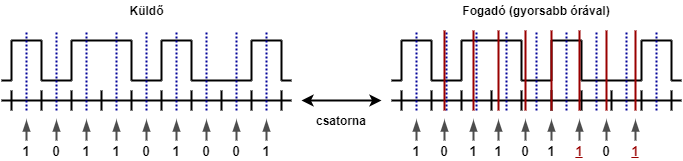
\includegraphics[width=0.8\textwidth]{img/szinkronizacio.png}
		\caption{Szinkronizáció szükségessége}
	\end{figure}

	\subsection*{Átviteli közegek}

	\paragraph{Vezetékes}

	\begin{itemize}[leftmargin=7.5mm]
        \renewcommand{\labelitemi}{$\vcenter{\hbox{\tiny$\bullet$}}$}
        \item \emph{Mágneses adathordozók}
	   \begin{itemize}[leftmargin=7.5mm]
            \renewcommand{\labelitemii}{$\vcenter{\hbox{\tiny$\circ$}}$}
            \item Nagy sávszélesség
            \item Nagy késletetés
        \end{itemize}
		\item \emph{Sodort érpár}
    	\begin{itemize}[leftmargin=7.5mm]
            \renewcommand{\labelitemii}{$\vcenter{\hbox{\tiny$\circ$}}$}
            \item Főként távbeszélőrendszerekben használatos
            \item Dupla rézhuzal
            \item Analóg és digitális jelátvitel
        \end{itemize}
		\item \emph{Koaxiális kábel}
    	\begin{itemize}[leftmargin=7.5mm]
            \renewcommand{\labelitemii}{$\vcenter{\hbox{\tiny$\circ$}}$}
            \item Nagyobb sebesség és távolság érhető el, mint a sodorttal
            \item Analóg és digitális jelátvitel
        \end{itemize}
        \item \emph{Fényvezető szálak (üvegszál)}
    	\begin{itemize}[leftmargin=7.5mm]
            \renewcommand{\labelitemii}{$\vcenter{\hbox{\tiny$\circ$}}$}
            \item Fényforrás, átviteli közeg és detektor
            \item Fényimpulzus 1-es bit, nincs	fényimpulzus 0-s bit
        \end{itemize}
    \end{itemize}

    \paragraph{Vezeték nélküli}

    \begin{itemize}[leftmargin=7.5mm]
        \renewcommand{\labelitemi}{$\vcenter{\hbox{\tiny$\bullet$}}$}
        \item \emph{Rádiófrekvenciás} átvitel
    	\begin{itemize}[leftmargin=7.5mm]
            \renewcommand{\labelitemii}{$\vcenter{\hbox{\tiny$\circ$}}$}
            \item Egyszerűen előállíthatóak
            \item Nagy távolságú átvitel (jel erősítés lehetséges)
            \item Kültéri és beltéri alkalmazhatóság \\
            \item Időjárás befolyásolhatja
            \item Lehallgathatóság
            \item Frekvenciakiosztás állami hatáskör
        \end{itemize}
        \item \emph{Mikrohullámú} átvitel
    	\begin{itemize}[leftmargin=7.5mm]
            \renewcommand{\labelitemii}{$\vcenter{\hbox{\tiny$\circ$}}$}
            \item Egyenes vonal mentén terjed
            \item Elhalkulás problémája
            \item Olcsó
        \end{itemize}
        \item \emph{Műholdas átvitel}
        \begin{itemize}
            \item 30.000 km felett keringő műholdak
            \item Eltérő frekvenciájú továbbítás, mint fogadás \\
            \item Időjárás függő
            \item Lehallgatható
            \item Nagy jel késés (a nagy távolság miatt)
        \end{itemize}
        \item \emph{Infravörös} és \emph{milliméteres hullámú} átvitel
    	\begin{itemize}[leftmargin=7.5mm]
            \renewcommand{\labelitemii}{$\vcenter{\hbox{\tiny$\circ$}}$}
            \item Kistávolságú átvitel esetén
            \item Szilárd tárgyakon nem hatol át
        \end{itemize}
        \item \emph{Látható fényhullámú} átvitel
    	\begin{itemize}[leftmargin=7.5mm]
            \renewcommand{\labelitemii}{$\vcenter{\hbox{\tiny$\circ$}}$}
            \item Lézerforrás + fényérzékelő
            \item Nagy sávszélesség,
            \item Nem engedélyköteles
            \item Biztonságos (nehezen lehallgatható)
            \item Olcsó \\
            \item Időjárás erősen befolyásolhatja
        \end{itemize}
        \item \emph{Bluetooth}
        \begin{itemize}[leftmargin=7.5mm]
            \renewcommand{\labelitemii}{$\vcenter{\hbox{\tiny$\circ$}}$}
            \item Kis hatótávolság (méterek),
            \item Adatcseréhez használható,
            \item Alacsony energiaszükséglet
        \end{itemize}
    \end{itemize}

	\subsection*{Jelátvitel\\}

	\begin{itemize}[leftmargin=7.5mm]
        \renewcommand{\labelitemi}{$\vcenter{\hbox{\tiny$\bullet$}}$}
		\item \textbf{Alapsáv}: A digitális jel direkt árammá vagy feszültséggé alakul. A jel minden frekvencián átvitelre kerül. Átviteli korlátok
		\begin{figure}[H]
			\centering
			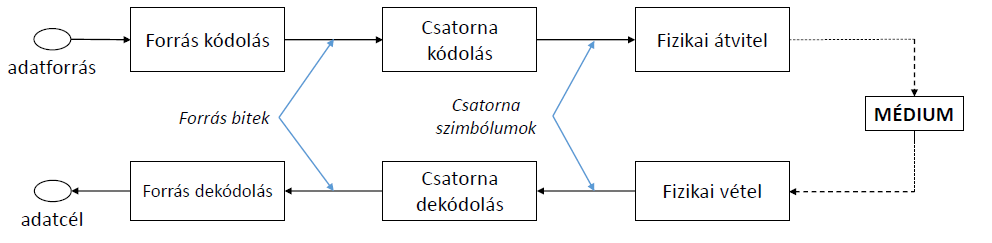
\includegraphics[width=1.0\textwidth]{img/alapsav.png}
			\caption{Digitális alapsávú átvitel struktúrája}
		\end{figure}
		\item \textbf{Szélessáv}: Széles frekvencia tartományban történik az átvitel.
		\begin{figure}[H]
			\centering
			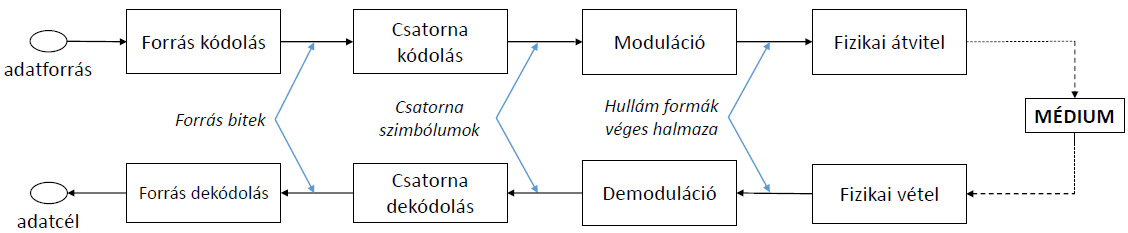
\includegraphics[width=1.0\textwidth]{img/szelessav.png}
			\caption{Digitális szélessávú átvitel struktúrája}
		\end{figure}
    \end{itemize}
    \noindent Modulációs eljárást alkalmazunk akkor, mikor a rendelkezésünkre álló átviteli közegen az átvinni kívánt információt hordozó jel nem képes, vagy csak nagy csillapítással, torzulással képes eljuttatni az egyik pontból egy másikba. Ekkor választunk egy olyan jelet (\emph{vivőjelet}), amelyet a rendelkezésre álló átviteli közeg az elvárásainknak megfelelően képes továbbítani.\\

    \noindent A modulációs eljárásokat megkülönböztetjük aszerint, hogy a vivő jel mely jellemzője fogja az információt eljuttatni egyik ponttól a másikig. Az információ továbbításához a vivő jel valamely jellemzőjét (esetleg jellemzőit) az információt hordozó jellel (\emph{moduláló jellel}) megváltoztatjuk. A fenti eljárást \textbf{modulációnak} nevezzük. A modulált jelet (vivőjel és moduláló jel segítségével előállított jel) eljuttatjuk az átviteli közegen keresztül a célpontig, majd leválasztjuk az információt hordozó jelet. A leválasztást nevezzük \textbf{demoduláció}nak.

    \section*{Modulációk}

        Egy szinuszos rezgés ábrázolása $T$ periódus idejű függvényre
        \[
            g(t)=Asin(2\pi f t + \varphi),\ ahol\ A\ \text{az amplitúdó}, f = \frac{1}{T}\ \text{a frekvencia és}\ \varphi\ \text{a fáziseltolás}.
        \]
        A jel modulálására az alábbi lehetőségeket használhatjuk.
						
        \paragraph*{Amplitúdó moduláció}

        Az $s(t)$ szignált a szinuszgörbe amplitúdójaként kódoljuk, azaz:
        \begin{align*}
            f_A(t) = s(t) \cdot sin(2\pi f t + \varphi)
        \end{align*}

	   \begin{itemize}[leftmargin=7.5mm]
            \renewcommand{\labelitemi}{$\vcenter{\hbox{\tiny$\bullet$}}$}
            \item Analóg szignál: amplitúdómoduláció
            \item Digitális szignál: amplitúdó keying\\
            (szignál erőssége egy diszkrét halmaz értékeinek megfelelően változik)
        \end{itemize}

        \begin{figure}[H]
            \centering
            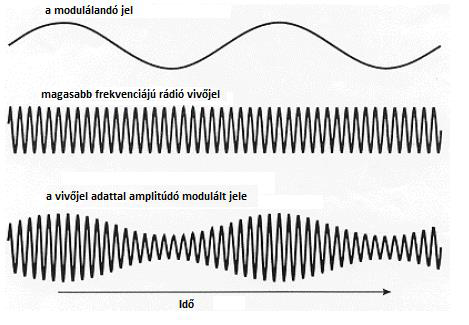
\includegraphics[width=0.5\textwidth]{img/amplitudo_mod.png}
            \caption{Amplitúdó moduláció}
        \end{figure}

        \begin{figure}[H]
            \centering
            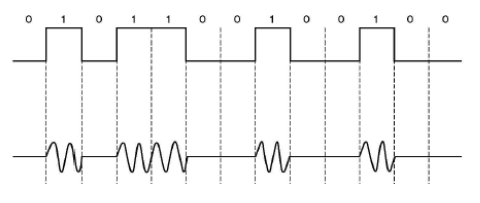
\includegraphics[width=0.6\textwidth]{img/amplitudo_key.png}
            \caption{Amplitúdó keying}
        \end{figure}

        \paragraph*{Frekvencia moduláció}

        Az $s(t)$ szignált a szinuszgörbe frekvenciájában kódoljuk, azaz:
        \begin{align*}
        	f_F(t) = a \cdot sin(2\pi s(t) t + \varphi)
        \end{align*}
        \begin{itemize}[leftmargin=7.5mm]
            \renewcommand{\labelitemi}{$\vcenter{\hbox{\tiny$\bullet$}}$}
            \item Analóg szignál: frekvenciamoduláció
            \item Digitális szignál: frekvencia-eltolás keying\\
            (például egy diszkrét halmaz szimbólumaihoz különböző frekvenciák hozzárendelésével)
        \end{itemize}
        \begin{figure}[H]
        	\centering
        	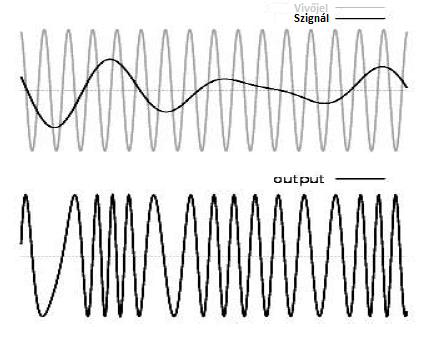
\includegraphics[width=0.5\textwidth]{img/frekvencia_mod.png}
        	\caption{Frekvencia moduláció}
        \end{figure}
        \begin{figure}[H]
        	\centering
        	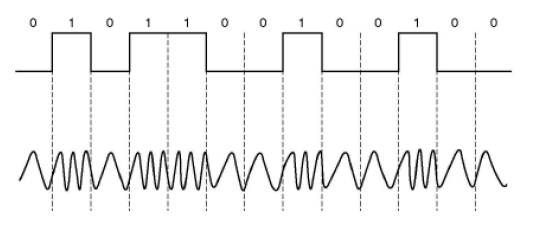
\includegraphics[width=0.6\textwidth]{img/frekvencia_key.png}
        	\caption{Frekvencia keying}	
        \end{figure}

        \paragraph*{Fázis moduláció}

        Az $s(t)$ szignált a szinuszgörbe fázisában kódoljuk, azaz:
        \begin{align*}
            f_P(t) = a \cdot sin(2\pi f t + s(t))
        \end{align*}
        \begin{itemize}[leftmargin=7.5mm]
            \renewcommand{\labelitemi}{$\vcenter{\hbox{\tiny$\bullet$}}$}
            \item Analóg szignál: fázis moduláció (nem igazán használják)
            \item Digitális szignál: fázis-eltolás keying\\
            (például egy diszkrét halmaz szimbólumaihoz különböző fázisok hozzárendelésével)
        \end{itemize}
        \begin{figure}[H]
        	\centering
        	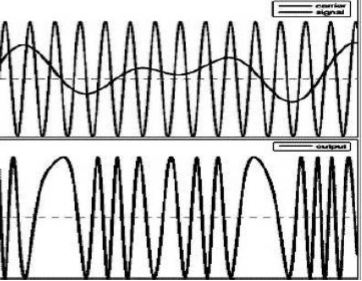
\includegraphics[width=0.5\textwidth]{img/fazis_mod.png}
        	\caption{Fázis moduláció}
        \end{figure}
        \begin{figure}[H]
        	\centering
        	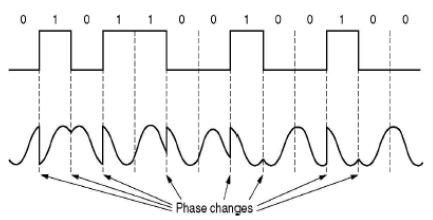
\includegraphics[width=0.6\textwidth]{img/fazis_key.png}
        	\caption{Fázis-eltolás keying}	
        \end{figure}
        \begin{itemize}[leftmargin=7.5mm]
            \renewcommand{\labelitemi}{$\vcenter{\hbox{\tiny$\bullet$}}$}
			\item Digitális és analóg jelek összehasonlítása: \\
            \begin{itemize}[leftmargin=7.5mm]
                \renewcommand{\labelitemii}{$\vcenter{\hbox{\tiny$\circ$}}$}
			    \item Digitális átvitel: Diszkrét szignálok véges halmazát használja.\\
                például: feszültség vagy áramerősség értékek.\\
			    \item Analóg átvitel: Szignálok folytonos halmazát használja.\\
                például: feszültség vagy áramerősség a vezetékben.\\
        \end{itemize}
    \end{itemize}

    \noindent Digitális esetében lehetőség van a vételpontosság helyreállítására illetve az eredeti jel helyreállítására, míg az analógnál a fellépő hibák önmagukat erősíthetik.

\newpage		
    \section*{2. Adatkapcsolati réteg}
		
	   Az adatkapcsolati réteg feladata jól definiált szolgálati interfész biztosítása a hálózati rétegnek, melynek három fázisa van:
        \begin{itemize}[leftmargin=7.5mm]
        \renewcommand{\labelitemi}{$\vcenter{\hbox{\tiny$\bullet$}}$}
            \item \emph{nyugtázatlan összeköttetés alapú} szolgálat
            \item \emph{nyugtázott összeköttetés nélküli} szolgálat
            \item \emph{nyugtázott összeköttetés alapú} szolgálat
        \end{itemize}
        Továbbá az átviteli hibák kezelése és az adatforgalom szabályozása (elárasztás elkerülése).

    \subsection*{Keretképzés\\}
        A fizikai réteg nem garantál hibamentességet, az adatkapcsolati réteg feladata a hibajelzés, illetve a szükség szerint javítás. \\

        \noindent Erre ad megoldást a keretekre tördelése a bitfolyamnak, és ellenőrző összegek számítása.\\
        A keretezés nem egyszerű feladat, mivel megbízható időzítésre nem nagyon van lehetőség.\\

        \noindent Négy lehetséges módszer:
        \begin{enumerate}
            \item \emph{\textbf{Karakterszámlálás}} \\\\
            A keretben lévő karakterek számát a keret fejlécében adjuk meg. Így a vevő adatkapcsolati rétege tudni fogja a keret végét. Probléma: nagyon érzékeny a hibára a módszer.
            \begin{figure}[H]
                \centering
                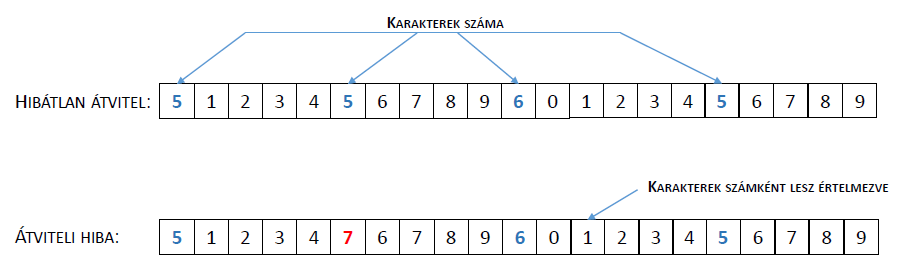
\includegraphics[width=0.75\textwidth]{img/karakterszamlalas.png}
                \caption{Karakterszámlálás}	
            \end{figure}

            \item \emph{\textbf{Kezdő és végkarakterek karakterbeszúrással}} \\\\
            Különleges bájtokat helyezünk el a keret elejének és végének jelzésére, aminek a neve jelző bájt (flagbyte). Az adatfolyamban szereplő speciális bájtokhoz ESC bájtot használnak.
            \begin{figure}[H]
                \centering
                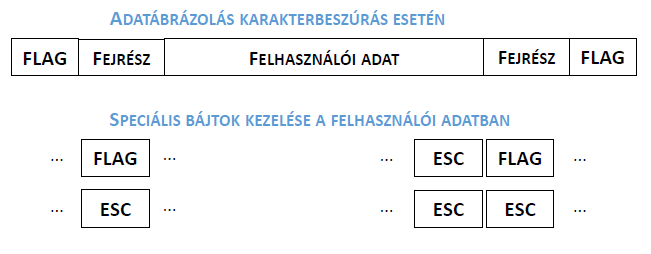
\includegraphics[width=0.6\textwidth]{img/karakterbeszuras.png}
                \caption{Kezdő és végkarakterek karakterbeszúrással}	
            \end{figure}
            \item \emph{\textbf{Kezdő és végjelek bitbeszúrása}} \\\\
            Minden keret egy speciális bitmintával kezdődik (flagbájt, 01111110) és minden egymást követő 5 hosszú folytonos 1-es bit sorozat után beszúr egy 0-át.
            \begin{figure}[H]
                \centering
                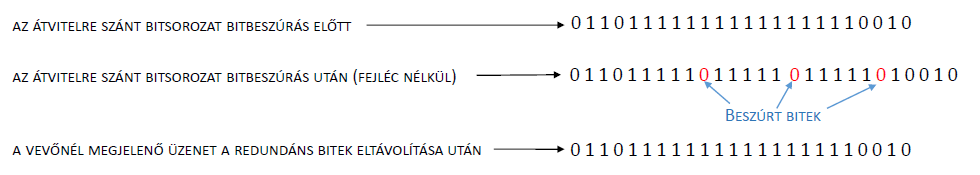
\includegraphics[width=1.0\textwidth]{img/bitbeszuras.png}
                \caption{Kezdő és végjelek bitbeszúrásal}	
            \end{figure}
            \item \emph{\textbf{Fizikai rétegbeli kódolás-sértés}} \\\\
            Olyan hálózatokban használható, ahol a fizikai rétegbeli kódolás redundanciát tartalmaz.
        \end{enumerate}

    \subsection*{Hibakezelés}

    Hibakezelés szempontjából a következő két esetet kell vizsgálnunk. A keretek megérkeztek-e a célállomás hálózati rétegéhez, illetve helyes sorrendben érkeztek-e meg. Ehhez valamilyen visszacsatolás szükséges a vevő és az adó között. (például nyugták). \\

    \noindent Időkorlátokat vezetünk be az egyes lépésekhez. Hiba estén a csomagot újraküldjük. Többszörös vétel lehet, amin segíthet a sorszámok használata.\\

    \noindent Az adatkapcsolati réteg feladata a hibakezelés szempontjából, hogy az időzítőket és számlálókat úgy kezelje, hogy biztosítani tudja a keretek pontosan egyszeri (nem több és nem kevesebb) megérkezését a célállomás hálózati rétegéhez.

    \subsubsection*{Bithibák}

    \begin{itemize}[leftmargin=5.5mm]
        \renewcommand{\labelitemi}{$\vcenter{\hbox{\tiny$\bullet$}}$}
        \item \textbf{\emph{Egyszerű bithiba}} \\\\
        Az adategység 1 bitje nulláról egyre avagy egyről nullára változik.
        \begin{figure}[H]
            \centering
            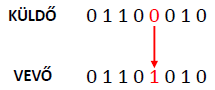
\includegraphics[width=0.2\textwidth]{img/egyszeru_bithiba.png}
            \caption{Egyszerű bithiba}	
        \end{figure}
        \item \textbf{\emph{Csoportos bithiba}} \\\\
        Egy olyan folytonos szimbólum sorozatot, amelynek az első és utolsó szimbóluma hibás, és nem létezik ezen két szimbólummal határolt részsorozatban olyan $m$ hosszú részsorozat, amelyet helyesen fogadtunk, $m$ hosszú csoportos bithibának nevezünk.

        \begin{figure}[H]
            \centering
            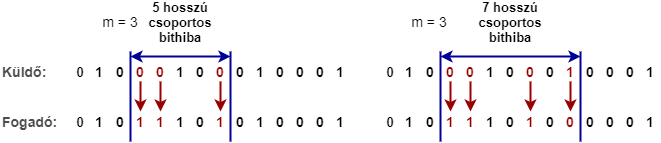
\includegraphics[width=1.0\textwidth]{img/csoportos_bithiba.png}
            \caption{Egyszerű bithiba}	
        \end{figure}

    \end{itemize}

    \subsection*{Hiba jelzés és javítás\\}

    Kétféle hibakezelési stratégia létezik:
    \begin{itemize}[leftmargin=7.5mm]
        \renewcommand{\labelitemi}{$\vcenter{\hbox{\tiny$\bullet$}}$}
        \item Hibajelző (redundáns információ mellékelése)
        \item Hibajavító kódok (adatok közé iktatott redundancia).
    \end{itemize}

    {\footnotesize \noindent \emph{Megjegyzés}: Megbízható csatornákon a hibajelzés olcsóbb. (csomagot inkább újraküldjük). A kevésbé megbízható csatornákon a hibajavításos módszer célszerűbb.}

    \paragraph*{Hamming-távolság, Hamming-korlát \\}

    \begin{itemize}[leftmargin=7.5mm]
        \renewcommand{\labelitemi}{$\vcenter{\hbox{\tiny$\bullet$}}$}
        \item Küldendő keret $m$ bitet tartalmaz.
        \item Redundáns bitek száma $r$.
        \item Az elküldött keret: $n = m+r$ bit.
    \end{itemize}

    \paragraph*{Hamming-távolság\\}

    Az olyan bitpozíciók számát, amelyeken a két kódszóban különböző bitek állnak, a két kódszó \emph{Hamming távolságának} nevezzük. Jelölés: $d(x,y)$\\

    \noindent Legyen $S$ az egyenlő hosszú bitszavak halmaza. $S$ Hamming-távolsága:
    \begin{align*}
        d(S) := \min_{x,y, \in S \ \land \ x \neq y} d(x,y)
    \end{align*}

    \noindent \textbf{d(S) = 1} esetén:\\

    \noindent Nincs hibafelismerés, ugyanis megengedett kódszóból 1 bit megváltoztatásával megengedett kódszó áll elő.
    \begin{figure}[H]
    	\centering
    	
\includegraphics[width=0.7\textwidth]{img/hamming1.png}
    	\caption{Kód Hamming-távolsága = 1}	
    \end{figure}
\newpage
    \noindent \textbf{d(S) = 2} esetén:\\

    \noindent Ha az $x$ kódszóhoz létezik olyan $v$ nem megengedett kódszó, amelyre $d(u,x)=1$, akkor hiba történt. Ha $x$ és $y$ megengedett kódszavak (távolságuk minimális = 2), akkor a következő összefüggésnek teljesülnie kell:

    \begin{align*}
        2 = d(x,y) \leq d(x,v)+d(v,y)
    \end{align*}

    \noindent Azaz egy bithiba felismerhető, de nem javítható.

    \begin{figure}[H]
    	\centering
    	
\includegraphics[width=0.7\textwidth]{img/hamming2.png}
    	\caption{Kód Hamming-távolsága = 2}	
    \end{figure}

    \noindent \textbf{d(S) = 3} esetén:\\

    \noindent Ekkor minden $u$, melyre $d(x,u)=1$ és $d(u,y) > 1$ nem megengedett.\\\\
    Ekkor három lehetőség áll fent:
    \begin{itemize}[leftmargin=7.5mm]
        \renewcommand{\labelitemi}{$\vcenter{\hbox{\tiny$\bullet$}}$}
        \item x került átvitelre és 1 bit hibával érkezett
    	\item y került átvitelre és 2 bit hibával érkezett
    	\item valami más került átvitelre és legalább 2 bit hibával érkezett
    \end{itemize}
    De valószínűbb, hogy $x$ került átvitelre, tehát ez egy 1 bit hiba javító, 2 bit hiba felismerő kód.
    \begin{figure}[H]
    	\centering
    	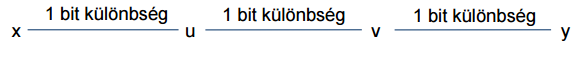
\includegraphics[width=0.6\textwidth]{img/hamming3.png}
    	\caption{Kód Hamming-távolsága = 3}	
    \end{figure}

    \paragraph*{Hamming-korlát\\}

    \noindent$ C \subseteq \{0,1\}^n$ és $d(C) = k$. Ekkor a kódszavak $\frac{k-1}{2}$ sugarú környezeteiben található bitszavak egymással diszjunkt halmazainak uniója legfeljebb az $n$-hosszú bitszavak halmazát adhatja ki.\\

    \noindent Formálisan:
    \[
        |C|\sum_{i=0}^{\lfloor\frac{k-1}{2}\rfloor}\dbinom{n}{i} \leq 2^n
    \]
    	
    \begin{itemize}[leftmargin=7.5mm]
        \renewcommand{\labelitemi}{$\vcenter{\hbox{\tiny$\bullet$}}$}
    	\item \emph{Hibafelismerés}: \\\\
        \textbf{$d$ bit hiba felismeréséhez} a keretek halmazában legalább $\textbf{d+1}$ Hamming távolság szükséges.
    	
    	\item \emph{Hibajavítás}: \\\\
        \textbf{$d$ bit hiba javításához} a megengedett keretek halmazában legalább $\textbf{2d+1}$ Hamming távolság szükséges.
    	
    	\item \emph{Kód rátája}: \\\\
        $R_S = \ddfrac{log_2|S|}{n}$ a kód rátája ($S \subseteq \{0,1\}^n$) - hatékonyságot karakterizálja
    	
    	\item \emph{Kód távolsága}: \\\\
        $\delta_S = \ddfrac{d(S)}{n}$ a kód távolsága  ($S \subseteq \{0,1\}^n$) - hibakezelést karakterizálja
    \end{itemize}
    A jó kódnak a rátája és a távolsága is nagy.

    \paragraph*{Paritásbit\\}

    A paritásbit olyan bit, melyet a kódszóban lévő egyesek száma alapján választunk.
    \begin{itemize}[leftmargin=7.5mm]
        \renewcommand{\labelitemi}{$\vcenter{\hbox{\tiny$\bullet$}}$}
    	\item \textbf{\small Odd Parity} (páratlan paritás): Az 1-esek száma páratlan. A kódszóban lévő 1-esek számát 1 vagy 0 hozzáadásával \emph{páratlanra egészítjük ki}.
    	\item \textbf{\small Even Parity} (páros paritás): Az 1-esek száma páros. A kódszóban lévő 1-esek számát 1 vagy 0 hozzáadásával \emph{párosra egészítjük ki}.
    \end{itemize}
    Egy paritást használó módszer az ún. Hamming módszer:
    \begin{itemize}
        \item A biteket 1-től sorszámozzuk balról, jobbra.
        \item Minden kettő-hatvány ($2^{i}$) helyen paritásbit van.
        \item Az egyes paritásbitek nem az összes bitet "ellenőrzik".
        \item A paritásbit ellenőrzi a teljes kódszó $i.$ bitjét, ha az $i$ kettes számrendszerbeli alakjában szerepel a $2^{i}$ helyiérték.\\
    \end{itemize}

    \noindent Például: a 6. bitet a 4-es és 2-es paritásbit ellenőrzi.\\

    \noindent A csoportok a következőképp alakulnak:
    \begin{itemize}[leftmargin=7.5mm]
        \renewcommand{\labelitemi}{$\vcenter{\hbox{\tiny$\bullet$}}$}
    	\item 1. bit: Minden első egyhosszú bitsorozat az első bittől kezdve (tehát: 1,3,5,7,...)
    	\item 2. bit: Minden első kéthosszú bitsorozat a második bittől kezdve (tehát: 2-3,6-7,10-11)
    	\item 4. bit: Minden első négyhosszú bitsorozat a negyedik bittől kezdve (tehát: 4-7,12-15)
    	\item stb.
    \end{itemize}
    \begin{figure}[H]
    	\centering
    	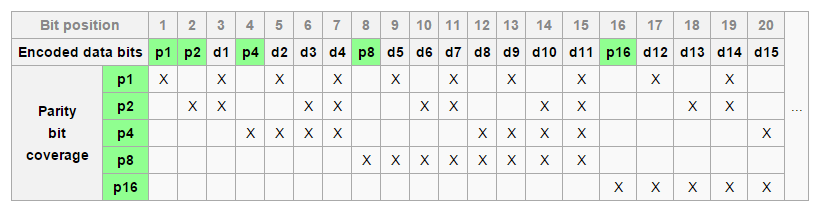
\includegraphics[width=0.9\textwidth]{img/paritasbit.png}
    	\caption{Paritásbitek csoportjai}	
    \end{figure}
    \newpage
    \noindent \emph{Példa}:\\

    \noindent Legyen az átküldendő üzenet: 1000101 \\

    \noindent Ekkor a kódszó a következőképp alakul: \\
    	{\color[rgb]{1,0,0}$\heartsuit\heartsuit$}1{\color[rgb]{1,0,0}$\heartsuit$}000{\color[rgb]{1,0,0}$\heartsuit$}101\\
    	A 8. bit a 8-11  bitsorozat paritását állítja be párosra:\\
    	{\color[rgb]{1,0,0}$\heartsuit\heartsuit$}1{\color[rgb]{1,0,0}$\heartsuit$}000{\color[rgb]{0,0,1}0101}\\
    	A 4. bit a 4-7  bitsorozat paritását állítja be párosra:\\
    	{\color[rgb]{1,0,0}$\heartsuit\heartsuit$}1{\color[rgb]{0,0,1}0000}0101\\
    	A 2. bit a 2-3, 6-7, 10-11 bitsorozat paritását állítja be párosra:\\
    	{\color[rgb]{1,0,0}$\heartsuit$}{\color[rgb]{0,0,1}01}00{\color[rgb]{0,0,1}00}01{\color[rgb]{0,0,1}01}\\
    	Az 1. bit az 1,3,5,7,9,11 bitsorozat paritását állítja be párosra: \\
    	{\color[rgb]{0,0,1}1}0{\color[rgb]{0,0,1}1}0{\color[rgb]{0,0,1}0}0{\color[rgb]{0,0,1}0}0{\color[rgb]{0,0,1}1}0{\color[rgb]{0,0,1}1}\\
    	
    \noindent Tehát a elküldendő bitsorozat:
    	{\color[rgb]{1,0,0}10}1{\color[rgb]{1,0,0}0}000{\color[rgb]{1,0,0}0}101\\

    \paragraph*{CRC - Polinom-kód, azaz ciklikus redundancia\\}

    A bitsorozatokat egy $\mathbb{Z}_2$ feletti polinom ($M(x)$) együtthatóinak tekintjük. \\
    Definiálunk egy $G(x)$ $r$-ed fokú generátorpolinomot, melyet a vevő és küldő egyaránt ismer.\\

    \noindent Algoritmus:
    \begin{enumerate}
    	\item Fűzzünk $r$ darab 0 bitet a keret alacsony helyi értékű végéhez. Azaz vegyük az $x^rM(x)$ polinomot (ez már $m+r$ fokú)
    	\item Osszuk el $x^rM(x)$-et $G(x)$-szel (mod 2).
    	\item A maradékot (mely mindig \emph{r} vagy kevesebb bitet tartalmaz) vonjuk ki \\
        $x^rM(x)$-ből (mod 2). Így az eredeti keret végére egy \emph{r} hosszú ellenőrző összeg kerül. Legyen ez a polinom $T(x)$.
    	\item A vevő egy $T(x)+E(x)$-nek megfelelő polinomot kap (ahol $E(x)$ a hiba polinom).\\
        Ezt elosztva a generátorpolinommal egy $R(x)$ polinomot kapunk. Ha ez a polinom nem nulla, akkor hiba történt.
    \end{enumerate}

    \noindent Áttekintés:
    \begin{itemize}[leftmargin=7.5mm]
        \renewcommand{\labelitemi}{$\vcenter{\hbox{\tiny$\bullet$}}$}
        \item $G(x)$ legmagasabb és legalacsonyabb fokú tagjának együtthatója mindig 1.
        \item A $G(x)$ többszöröseinek megfelelő bithibákat nem ismeri fel, azaz, ha
        \begin{center}
            $\forall j \in \mathbb{N}: E(x) = x^jG(x)$
        \end{center}
        \item Szerkeszthető egy egyszerű, léptető regiszteres áramkör az ellenőrző összeg hardverben történő kiszámítására és ellenőrzésére.
    \end{itemize}
    \newpage

    \noindent Példa: Legyen az
    \begin{itemize}[leftmargin=7.5mm]
        \renewcommand{\labelitemi}{$\vcenter{\hbox{\tiny$\bullet$}}$}
        \item átküldendő üzenet: 11010011100
        \item $G(x) = x^3 + x + 1 = \textbf{1} x^3 + \textbf{0} x^2 + \textbf{1} x^1 + \textbf{1} x^0 = x^3 + x + 1 \quad \rightarrow \textbf{r = 3}$
    \end{itemize}

    \noindent Minden lépésben a következő 1-es alá írom a generátorpolinomot első 1-sét, és ha két egyforma érték van egymás alatt, nullát írok alá, különben 1-et.    \\

    $\begin{array}{cccccccccccccc|l}
        1&1&0&1&0&0&1&1&1&0&0& & & &\text{\small eredeti üzenet} \\
        1&1&0&1&0&0&1&1&1&0&0&0&0&0&\text{\small r darab 0-val kiegészítve} \\
        1&0&1&1& & & & & & & & & & &\text{\small generátor polinommal osztás} \\
        0&1&1&0&0&0&1&1&1&0&0&0&0&0&\text{\small eredmény} \\
         &1&0&1&1& & & & & & & & & &\text{\small generátor polinommal osztás} \\
        0&0&1&1&1&0&1&1&1&0&0&0&0&0& \cdots \\
         & &1&0&1&1& & & & & & & & &  \\
        0&0&0&1&0&1&1&1&1&0&0&0&0&0&  \\
         & & &1&0&1&1& & & & & & & &  \\
        0&0&0&0&0&0&0&1&1&0&0&0&0&0&  \\
         & & & & & & &1&0&1&1& & & &  \\
        0&0&0&0&0&0&0&0&1&1&1&0&0&0&  \\
         & & & & & & & &1&0&1&1& & &  \\
        0&0&0&0&0&0&0&0&0&1&0&1&0&0&  \\
        & & & & & & & & & 1&0&1&1& &  \\
        0&0&0&0&0&0&0&0&0&0&0&0&1&0&  \\
    \end{array}$\\\\

    \noindent Az utolsó $r(=3)$ bitet hozzáfüzzük az eredeti üzenethez: 11010011100\textbf{010}\\

    \noindent Ellenőrzés a vevő oldalon:\\

    $\begin{array}{cccccccccccccc|l}
        1&1&0&1&0&0&1&1&1&0&0&0&1&0&\text{\small kódolt üzenet} \\
        1&0&1&1& & & & & & & & & & &\text{\small generátor polinommal osztás} \\
        0&1&1&0&0&0&1&1&1&0&0&0&1&0&\text{\small eredmény} \\
         &1&0&1&1& & & & & & & & & &\text{\small generátor polinommal osztás} \\
        0&0&1&1&1&0&1&1&1&0&0&0&1&0& \cdots \\
         & &1&0&1&1& & & & & & & & &  \\
        0&0&0&1&0&1&1&1&1&0&0&0&1&0&  \\
         & & &1&0&1&1& & & & & & & &  \\
        0&0&0&0&0&0&0&1&1&0&0&0&1&0&  \\
         & & & & & & &1&0&1&1& & & &  \\
        0&0&0&0&0&0&0&0&1&1&1&0&1&0&  \\
         & & & & & & & &1&0&1&1& & &  \\
        0&0&0&0&0&0&0&0&0&1&0&1&1&0&  \\
        & & & & & & & & & 1&0&1&1& &  \\
        0&0&0&0&0&0&0&0&0&0&0&0&0&0&  \\
    \end{array}$\\\\

    \noindent Minden bit 0 lett, azaz az üzenet nem sérült.

\newpage
	\subsection*{Protokollok}

    \subsubsection*{Elemi adatkapcsolati protokollok\\}

    \noindent Feltevések:
     \begin{itemize}[leftmargin=7.5mm]
        \renewcommand{\labelitemi}{$\vcenter{\hbox{\tiny$\bullet$}}$}
        \item A fizikai, az adatkapcsolati és a hálózati réteg független folyamatok, amelyek üzeneteken keresztül kommunikálnak egymással.
        \item Az \emph{A} gép megbízható, összeköttetés alapú szolgálat alkalmazásával akar a \emph{B} gépnek egy hosszú adatfolyamot küldeni. (Adatok előállítására sosem kell várnia \emph{A} gépnek.)
        \item A gépek nem fagynak le.
        \item Adatkapcsolati fejrészben vezérlési információk.
        \item Adatkapcsolati lábrészben ellenőrző összeg.
    \end{itemize}

    \noindent Kommunikáció fajtái:
     \begin{itemize}[leftmargin=7.5mm]
        \renewcommand{\labelitemi}{$\vcenter{\hbox{\tiny$\bullet$}}$}
        \item szimplex kommunikáció – a kommunikáció pusztán egy irányba lehetséges
        \item fél-duplex kommunikáció – mindkét irányba folyhat kommunikáció, de egyszerre csak egy irány lehet aktív.
        \item duplex kommunikáció – mindkét irányba folyhat kommunikáció szimultán módon\\\
    \end{itemize}

    \noindent \textbf{\small Az összes protokoll esetében}
    \begin{itemize}
        \item Résztvevők: küldő és vevő
    \end{itemize}

  	\paragraph*{Korlátozás nélküli szimplex protokoll\\}

    \textbf{\small A környezet}
    \begin{itemize}[leftmargin=7.5mm]
        \renewcommand{\labelitemi}{$\vcenter{\hbox{\tiny$\bullet$}}$}
        \item Mind az adó, mind a vevő hálózati rétegei mindig készen állnak
        \item A feldolgozási időktől eltekintünk
        \item Végtelen puffer-területet feltételezünk
        \item Az adatkapcsolati rétegek közötti kommunikációs csatorna sosem rontja/veszíti el a\\
        kereteket
    \end{itemize}

    \noindent \textbf{\small A protokoll}
    \begin{itemize}[leftmargin=7.5mm]
        \renewcommand{\labelitemi}{$\vcenter{\hbox{\tiny$\bullet$}}$}
        \item Nincs sem sorszámozás, sem nyugta (szimplex)
        \item A küldő végtelen ciklusban küldi kifelé a kereteket folyamatosan
        \item A vevő kezdetben várakozik az első keret megérkezésére, keret érkezésekor a hardver puffer tartalmát változóba teszi és az adatrészt tovább küldi a hálózati rétegnek
    \end{itemize}

    \paragraph*{Szimplex megáll és vár protokoll}

    \textbf{\small A környezet}
    \begin{itemize}[leftmargin=7.5mm]
        \renewcommand{\labelitemi}{$\vcenter{\hbox{\tiny$\bullet$}}$}
        \item Mind az adó, mind a vevő hálózati rétegei mindig készen állnak
        \item A vevőnek $\Delta t$ időre van szüksége a bejövő keret feldolgozására
        \subitem nincs pufferelés és sorban állás sem
        \item Az adatkapcsolati rétegek közötti kommunikációs csatorna sosem rontja/veszíti el a\\
        kereteket
    \end{itemize}

    \noindent \textbf{\small A protokoll}
    \begin{itemize}[leftmargin=7.5mm]
        \renewcommand{\labelitemi}{$\vcenter{\hbox{\tiny$\bullet$}}$}
        \item A küldő egyesével küldi kereteket és addig nem küld újat, még nem kap nyugtát a vevőtől (fél-duplex)
        \item A vevő kezdetben várakozik az első keret megérkezésére, keret érkezésekor a hardver puffer tartalmát változóba teszi és az adatrészt továbbküldi a hálózati rétegnek, végül nyugtázza a keretet
    \end{itemize}

    \paragraph*{Szimplex protokoll zajos csatornához}
    \textbf{\small A környezet}
    \begin{itemize}[leftmargin=7.5mm]
        \renewcommand{\labelitemi}{$\vcenter{\hbox{\tiny$\bullet$}}$}
    	\item Mind az adó, mind a vevő hálózati rétegei mindig készen állnak
        \item A vevőnek $\Delta t$ időre van szüksége a bejövő keret feldolgozására
        \subitem nincs pufferelés és sorban állás sem
    	\item Az adatkapcsolati rétegek közötti kommunikációs csatorna hibázhat
        \subitem keret megsérülése vagy elvesztése
    \end{itemize}
    	 	
    \noindent \textbf{\small A protokoll}
    \begin{itemize}[leftmargin=7.5mm]
        \renewcommand{\labelitemi}{$\vcenter{\hbox{\tiny$\bullet$}}$}
    	\item A küldő egyesével küldi kereteket és addig nem küld újat, még nem kap nyugtát a vevőtől egy megadott határidőn belül, ha a határidő lejár, akkor ismételten elküldi az aktuális keretet.
    	\item A vevő kezdetben várakozik az első keret megérkezésére, keret érkezésekor a hardver puffer tartalmát változóba teszi, leellenőrzi a kontroll összeget:
    	\begin{itemize}
    		\item Nincs hiba: az adatrészt továbbküldi a hálózati rétegnek, végül nyugtázza a keretet.
    		\item Hiba történt: eldobja a keretet és nem nyugtáz (duplikátumok kellenek)
    	\end{itemize}
    \end{itemize}

    \paragraph*{Csúszóablakos protokoll}

    \noindent Alapok (általános):
    \begin{itemize}[leftmargin=7.5mm]
        \renewcommand{\labelitemi}{$\vcenter{\hbox{\tiny$\bullet$}}$}
        \item Egy adott időpontban egyszerre több keret is átviteli állapotban lehet
        \item A fogadó $n$ keretnek megfelelő méretű puffert allokál
        \item A küldőnek legfeljebb $n$, azaz ablak méretnyi, nyugtázatlan keret küldése engedélyezett
        \item A keret sorozatbeli pozíciója adja a keret címkéjét (sorozatszám)\\
    \end{itemize}

    \noindent Alapok (fogadó):
    \begin{itemize}[leftmargin=7.5mm]
        \renewcommand{\labelitemi}{$\vcenter{\hbox{\tiny$\bullet$}}$}
        \item A keret nyugtázója tartalmazza a következőnek várt keret sorozatszámát.
        \begin{itemize}[leftmargin=7.5mm]
            \renewcommand{\labelitemii}{$\vcenter{\hbox{\tiny$\circ$}}$}
            \item kumulatív nyugta – Olyan nyugta, amely több keretet nyugtáz egyszerre. Például, ha a 2,3 és 4 kereteket is fogadnánk, akkor a nyugtát 5 sorszám tartalommal küldenénk, amely nyugtázza mind a három keretet.
        \end{itemize}
        \item A hibás kereteket el kell dobni.
        \item A nem megengedett sorozatszámmal érkező kereteket el kell dobni.\\
    \end{itemize}

    \noindent Jellemzők (általános):
    \begin{itemize}[leftmargin=7.5mm]
        \renewcommand{\labelitemi}{$\vcenter{\hbox{\tiny$\bullet$}}$}
        \item A küldő nyilvántartja a küldhető sorozatszámok halmazát. (adási ablak)
        \item A fogadó nyilvántartja a fogadható sorozatszámok halmazát. (vételi ablak)
        \item A sorozatszámok halmaza minden esetben véges.
        \begin{itemize}[leftmargin=7.5mm]
            \renewcommand{\labelitemii}{$\vcenter{\hbox{\tiny$\circ$}}$}
            \item $K$ bites mező esetén: $[0..2K-1]$
        \end{itemize}
        \item A adási ablak minden küldéssel szűkül, illetve nő egy nyugta érkezésével.\\
        \end{itemize}

    \noindent Jellemzők (gyakorlati alkalmazás esetén):
    \begin{itemize}[leftmargin=7.5mm]
        \renewcommand{\labelitemi}{$\vcenter{\hbox{\tiny$\bullet$}}$}
        \item A gyakorlatban kétirányú adatfolyamot kell kezelni (duplex csatorna)
        \begin{itemize}[leftmargin=7.5mm]
            \renewcommand{\labelitemii}{$\vcenter{\hbox{\tiny$\circ$}}$}
                \item két különböző szimplex csatorna használata (két áramkör használata)
                \item egy csatorna használata (egy áramkör használata)
                \begin{itemize}[leftmargin=7.5mm]
                    \renewcommand{\labelitemiii}{$\vcenter{\hbox{\tiny$\diamond$}}$}
                    \item piggybacking módszer– a kimenő nyugtákat késleltetjük, hogy rá tudjuk akasztani a következő kimenő adatkeretre (ack mező használata)
                \end{itemize}
        \end{itemize}
    \end{itemize}

    \noindent Mi van ha egy hosszú folyam közepén történik egy keret hiba?
    \begin{itemize}[leftmargin=7.5mm]
        \renewcommand{\labelitemi}{$\vcenter{\hbox{\tiny$\bullet$}}$}
    	\item \textbf{\small "visszalépés N-nel" stratégia}
        \item[] Stratégia:
        \begin{itemize}[leftmargin=7.5mm]
            \renewcommand{\labelitemii}{$\vcenter{\hbox{\tiny$\circ$}}$}
            \item Az összes hibás keret utáni keretet eldobja és nyugtát sem küld róluk.
            \item Mikor az adónak lejár az időzítője, akkor újraküldi az összes nyugtázatlan keretet, kezdve a sérült vagy elveszett kerettel.
        \end{itemize}
        \item[] Következmények:
        \begin{itemize}[leftmargin=7.5mm]
            \renewcommand{\labelitemii}{$\vcenter{\hbox{\tiny$\circ$}}$}
            \item Egy méretű vételi ablakot feltételez.
            \item Nagy sávszéleséget pazarolhat el, ha nagy a hibaarány.
        \end{itemize}
\newpage        
    	\item \textbf{\small "szelektív ismétlés" stratégia}
        \item[] Stratégia:
        \begin{itemize}[leftmargin=7.5mm]
            \renewcommand{\labelitemii}{$\vcenter{\hbox{\tiny$\circ$}}$}
            \item A hibás kereteket eldobja, de a jó kereteket a hibás után puffereli.
            \item Mikor az adónak lejár az időzítője, akkor a legrégebbi nyugtázatlan keretet küldi el újra.
        \end{itemize}
        \item[] Következmények:
        \begin{itemize}[leftmargin=7.5mm]
            \renewcommand{\labelitemii}{$\vcenter{\hbox{\tiny$\circ$}}$}
            \item Javíthat a hatékonyságon a negatív nyugta használata. (NAK)
            \item Egynél nagyobb méretű vételi ablakot feltételezünk.
            \item Nagy memória igény, ha nagy vételi ablak esetén.\\\\
        \end{itemize}
    \end{itemize}

    \subsection*{Példák adatkapcsolati protokollokra}

    \begin{itemize}[leftmargin=7.5mm]
        \renewcommand{\labelitemi}{$\vcenter{\hbox{\tiny$\bullet$}}$}
    	\item \textbf{\small HDLC - High-level Data Link Control} \\
        A HDLC protokoll 3 bites csúszó-ablak protokollt alkalmaz  a sorszámozáshoz.\\
        Három típusú keretet használ:
        \begin{itemize}[leftmargin=7.5mm]
            \renewcommand{\labelitemii}{$\vcenter{\hbox{\tiny$\circ$}}$}
        	\item információs
        	\item felügyelő
        	\begin{itemize}[leftmargin=7.5mm]
            \renewcommand{\labelitemiii}{$\vcenter{\hbox{\tiny$\diamond$}}$}
                \item nyugtakeret (RECIEVE READY)
                \item negatív nyugta keret (REJECT)
                \item vételre nem kész (RECIEVE NOT READY) - nyugtáz minden keretet a következőig
                \item szelektív elutasítás (SELECTIVE REJECT) - egy gy adott keret újraküldésére szólít fel
        	\end{itemize}
        	\item Számozatlan
        \end{itemize}

    Általános keretfelépítése:
    \begin{itemize}[leftmargin=7.5mm]
        \renewcommand{\labelitemii}{$\vcenter{\hbox{\tiny$\circ$}}$}
      	\item FLAG bájt a keret határok jelzésére
       	\item \textit{cím} mező - több vonallal rendelkező terminálok esetén van jelentősége
       	\item \textit{vezérlés} mező - sorszámozás, nyugtázás és egyéb feladatok ellátására
       	\item \textit{adat} mező - tetszőleges hosszú adat lehet
       	\item \textit{ellenőrző összeg} mező - CRC kontrollösszeg  (CRC-CCITT generátor polinom felhasználásával)
    \end{itemize}
    \begin{figure}[H]
       	\centering
       	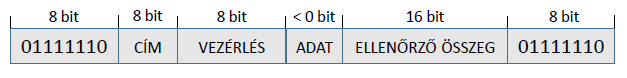
\includegraphics[width=0.8\textwidth]{img/hdlc_keret.png}
       	\caption{HDLC keret felépítése}	
    \end{figure}
\newpage
    \item \textbf{\small PPP - Point-to Point Protocol} \\

    A PPP protokoll három dolgot biztosít:
    \begin{itemize}[leftmargin=7.5mm]
        \renewcommand{\labelitemii}{$\vcenter{\hbox{\tiny$\circ$}}$}
        \item  Keretezési módszert (egyértelmű kerethatárok)
        \item Kapcsolatvezérlő protokollt (a vonalak felélesztésére, tesztelésére, az opció egyeztetésére és a vonalak elengedésére.)
        \item Olyan módot a hálózati réteg-opciók megbeszélésére, amely független az alkalmazott hálózati réteg-protokolltól.
            \begin{figure}[H]
                \centering
                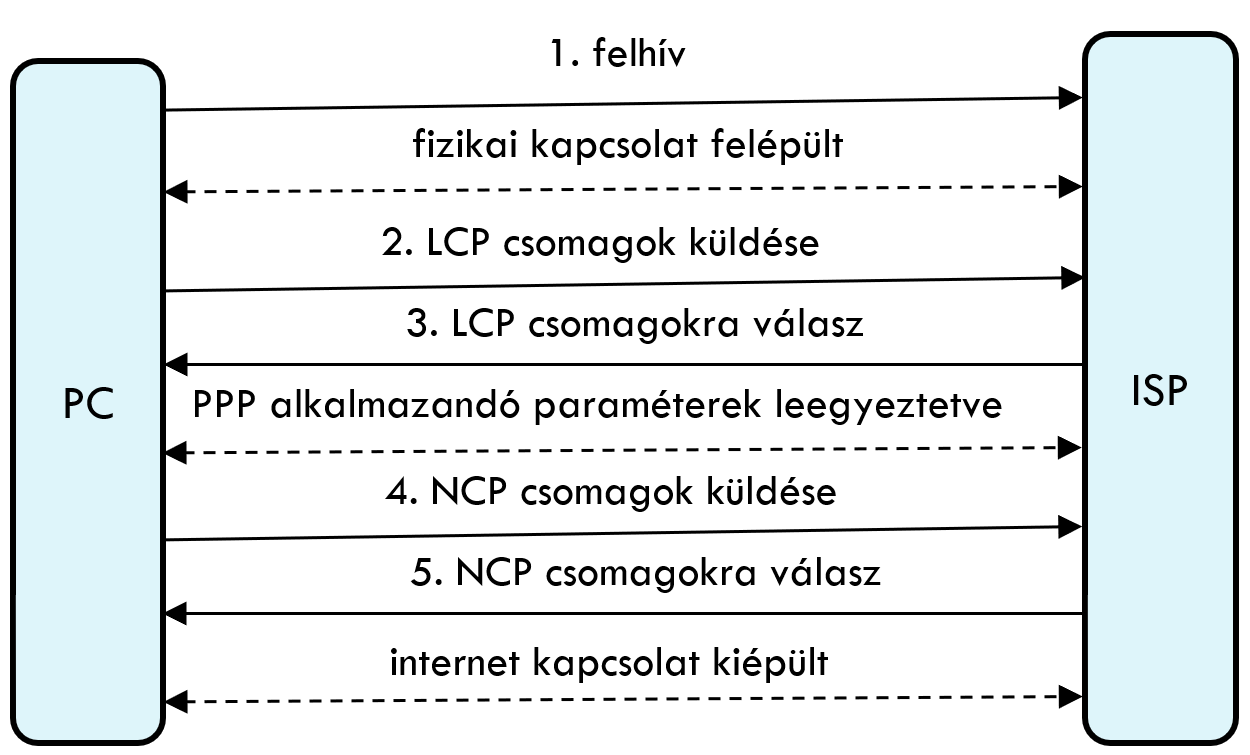
\includegraphics[width=0.65\textwidth]{img/ppp.png}
                \caption{}	
            \end{figure}
        \end{itemize}
        Bájt alapú keretszerkezet használ (azaz a legkisebb adategység a bájt).
        Vezérlő mező alapértéke a számozatlan keretet jelzi. Protokoll mezőben protokoll kód lehet az LCP, NCP, IP, IPX, AppleTalk vagy más protokollhoz.
        \begin{figure}[H]
        	\centering
        	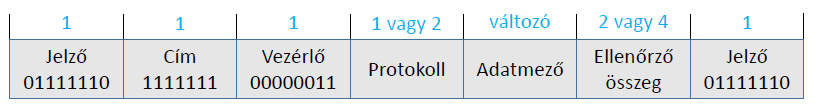
\includegraphics[width=0.8\textwidth]{img/ppp_keret.png}
        	\caption{PPP keret felépítése}	
        \end{figure}
    \end{itemize}
   	
   \paragraph*{MAC - Media Access Control\\}

    Egyetlen üzenetszórásos csatorna megosztása több egymással versengő felhasználó (állomás) között. A csatorna kiosztás történhet statikus vagy dinamikus módon.

    \subsubsection*{Statikus csatornamegosztási módszerek}

    \noindent Statikus esetben vagy frekvenciaosztásos nyalábolást vagy időosztásos nyalábolást használnak.
    \begin{itemize}[leftmargin=7.5mm]
        \renewcommand{\labelitemi}{$\vcenter{\hbox{\tiny$\bullet$}}$}
        \item Frekvenciaosztásos (FDM) esetben
        \begin{itemize}[leftmargin=7.5mm]
            \renewcommand{\labelitemii}{$\vcenter{\hbox{\tiny$\circ$}}$}
            \item A sávszélességet osztják $n$ egyenlő részre, és mindegyik felhasználó egy sávot kap.
            \item Mindenkinek külön frekvenciasávja van, így nincs interferencia.
        \end{itemize}
        \item Időosztásos (TDM) esetben
        \begin{itemize}[leftmargin=7.5mm]
            \renewcommand{\labelitemii}{$\vcenter{\hbox{\tiny$\circ$}}$}
            \item Az időegységet osztják $n$ egyenlő időrésre.
            \item Minden felhasználóhoz statikusan egy időrést rendel.\\
            (Az i. részben az i. felhasználó a teljes sávszélességet használhatja)
        \end{itemize}
    \end{itemize}

    \noindent Jellemzőik:
    \begin{itemize}[leftmargin=7.5mm]
        \renewcommand{\labelitemi}{$\vcenter{\hbox{\tiny$\bullet$}}$}
        \item kötött a felhasználószám
        \item a keretek átlagos késleltetése n-szerese annak, mintha az egész csatorna egy felhasználóé lenne
        \begin{itemize}[leftmargin=7.5mm]
            \renewcommand{\labelitemii}{$\vcenter{\hbox{\tiny$\circ$}}$}
            \item FDM-nél kisebb (n-ed része) sávszélesség,
            \item TDM-nél nagyobb várakozási idő van\\
            (a ciklusidő n-ed része csak az övé).
        \end{itemize}
        \item a keretek késleltetése állandó
        \item a csatornakihasználtság
        \begin{itemize}[leftmargin=7.5mm]
            \renewcommand{\labelitemii}{$\vcenter{\hbox{\tiny$\circ$}}$}
            \item rossz kis és nem egyenletes forgalom esetén\\
            (ha foglalt csatorna üres, más akkor sem veheti át)
            \item jó folytonos, egyenletes terheléskor\\
            (pl. telefonközpontközi trönk – kevés rögzített számú felhasználó, nagy egyenletes terhelés).
        \end{itemize}
    \end{itemize}

    \subsection*{Dinamikus csatornamegosztási módszerek}

    \subsubsection*{Verseny protokollok\\}

    $N$ független állomás van, amelyeken egy program vagy egy felhasználó továbbítandó kereteket generál. Ha egy állomás generált egy keretet, akkor blokkolt állapotban marad mindaddig, amíg a keretet sikeresen nem továbbította. Egyetlen csatorna van, melyen mindenféle kommunikáció zajlik. Minden állomás tud adatot küldeni és fogadni ezen a csatornán. Ha két keret egy időben kerül átvitelre, akkor átlapolódnak, és az eredményül kapott jel értelmezhetetlenné válik. Ezt nevezzük ütközésnek. Ez minden állomás számára felismerhető. Az ütközésben érintett kereteket később újra kell küldeni. (Ezen a hibán kívül egyéb hiba nem történhet.)\\

    \noindent Kétféle időmodellt különböztetünk meg:
    \begin{enumerate}
        \item \textbf{\small Folytonos} – Mindegyik állomás tetszőleges időpontban megkezdheti a küldésre kész keretének sugárzását.
        \item \textbf{\small Diszkrét} – Az időt diszkrét résekre osztjuk. Keret továbbítás csak időrés elején lehetséges. Az időrés lehet üres, sikeres vagy ütközéses
    \end{enumerate}

    \noindent Az egyes állomások vagy rendelkeznek vivőjel érzékeléssel vagy nem.
    \begin{itemize}[leftmargin=7.5mm]
        \renewcommand{\labelitemi}{$\vcenter{\hbox{\tiny$\bullet$}}$}
        \item Ha nem, akkor az állomások nem tudják megvizsgálni a közös csatorna állapotát, ezért egyszerűen elkezdenek küldeni, ha van rá lehetőségük.
        \item Ha igen, akkor az állomások meg tudják vizsgálni a közös csatorna állapotát a küldés előtt. A csatorna lehet: foglalt vagy szabad. Ha a foglalt a csatorna, akkor nem próbálják használni az állomások, amíg fel nem szabadul
    \end{itemize}

    \paragraph*{Egyszerű ALOHA \\}

    \begin{itemize}[leftmargin=7.5mm]
        \renewcommand{\labelitemi}{$\vcenter{\hbox{\tiny$\bullet$}}$}
        \item A felhasználó akkor vihet át adatot, amikor csak szeretne.
        \item Ütközés esetén véletlen ideig várakozik az állomás, majd újra próbálkozik.
        \item Keret idő–egy szabványos, fix hosszúságú keret átviteléhez szükséges idő (T).
        \item Egy keret akkor nem szenved ütközést, ha elküldésének első pillanatától kezdve egy keretideig nem próbálkozik más állomás keretküldéssel.
        \item 2T ideig ütközésveszélyes.
    \end{itemize}
    \begin{figure}[H]
        \centering
        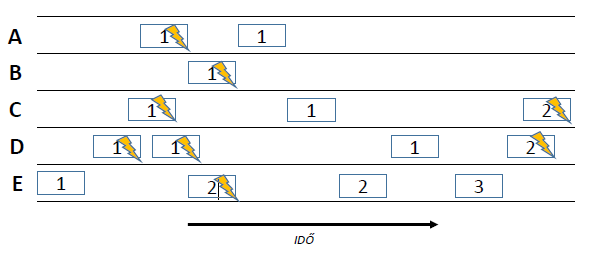
\includegraphics[width=0.7\textwidth]{img/egyszeru_aloha.png}
        \caption{Egyszerű ALOHA keret ütközések}	
    \end{figure}

    \paragraph*{Réselt ALOHA \\}

    \begin{itemize}[leftmargin=7.5mm]
        \renewcommand{\labelitemi}{$\vcenter{\hbox{\tiny$\bullet$}}$}
        \item Az időt keretidőnyi (T) résekre osztják
        \begin{itemize}[leftmargin=7.5mm]
            \renewcommand{\labelitemii}{$\vcenter{\hbox{\tiny$\circ$}}$}
            \item külön meg kell oldani az állomások szinkronizációját, pl. egy külön állomás küld egy speciális jelet minden rés elején.
        \end{itemize}
        \item Adást csak az időrés elején lehet kezdeni!
        \item Az ütközésveszélyes kritikus időszakasz 2T-ről T-re csökken az egyszerű ALOHA-hoz képest.
    \end{itemize}

    \paragraph*{1-prezisztens CSMA \\}

    Vivőjel érzékelés van, azaz minden állomás belehallgathat a csatornába. Folytonos időmodellt használ a protokoll. \\

    \noindent Algoritmus:
    \begin{enumerate}	
    	\item Keret leadása előtt belehallgat a csatornába:
    	\begin{enumerate}
                \item Ha foglalt, akkor addig vár, amíg fel nem szabadul. Szabad csatorna esetén azonnal küld. (perzisztens)
                \item Ha szabad, akkor küld.
    	\end{enumerate}
    	\item Ha ütközés történik, akkor az állomás véletlen hosszú ideig vár, majd újrakezdi a keret leadását.
     \end{enumerate}

    \paragraph*{Nem-prezisztens CSMA}

    Vivőjel érzékelés van, azaz minden állomás belehallgathat a csatornába. Folytonos időmodellt használ a protokoll. Mohóságot kerüli, azaz nem küld azonnal, ha foglalt.\\

    \noindent Algoritmus:
    \begin{enumerate}	
    	\item Keret leadása előtt belehallgat a csatornába:
    	\begin{enumerate}
                \item Ha foglalt, akkor véletlen ideig vár (nem figyeli a forgalmat), majd kezdi előröl a küldési algoritmust. (nem-perzisztens)
                \item Ha szabad, akkor küld.
    	\end{enumerate}
    	\item Ha ütközés történik, akkor az állomás véletlen hosszú ideig vár, majd újrakezdi a keret leadását.
    \end{enumerate}

    \paragraph*{p-prezisztens CSMA}

    Vivőjel érzékelés van, azaz minden állomás belehallgathat a csatornába. Diszkrét időmodellt használ a protokoll.\\

    \noindent Algoritmus:
    \begin{enumerate}	
    	\item Adás kész állapotban az állomás belehallgat a csatornába:
    	\begin{enumerate}
                \item Ha foglalt, akkor vár a következő időrésig, majd megismétli az algoritmust.
                \item Ha szabad, akkor $p$ valószínűséggel küld, illetve $1-p$ valószínűséggel visszalép a szándékától a következő időrésig. Várakozás esetén a következő időrésben megismétli az algoritmust. Ez addig folytatódik, amíg el nem küldi a keretet, vagy amíg egy másik állomás el nem kezd küldeni, mert ilyenkor úgy viselkedik, mintha ütközés történt volna.
    	\end{enumerate}
    	\item Ha ütközés történik, akkor az állomás véletlen hosszú ideig vár, majd újrakezdi a keret leadását.
    \end{enumerate}

    \paragraph*{CSMA/CD}

    Ütközés érzékelés esetén meg lehessen szakítani az adást. Minden állomás küldés közben megfigyeli a csatornát, ha ütközést tapasztalna, akkor megszakítja az adást, és véletlen ideig várakozik, majd újra elkezdi leadni a keretét.

    \begin{figure}[H]
        	\centering
        	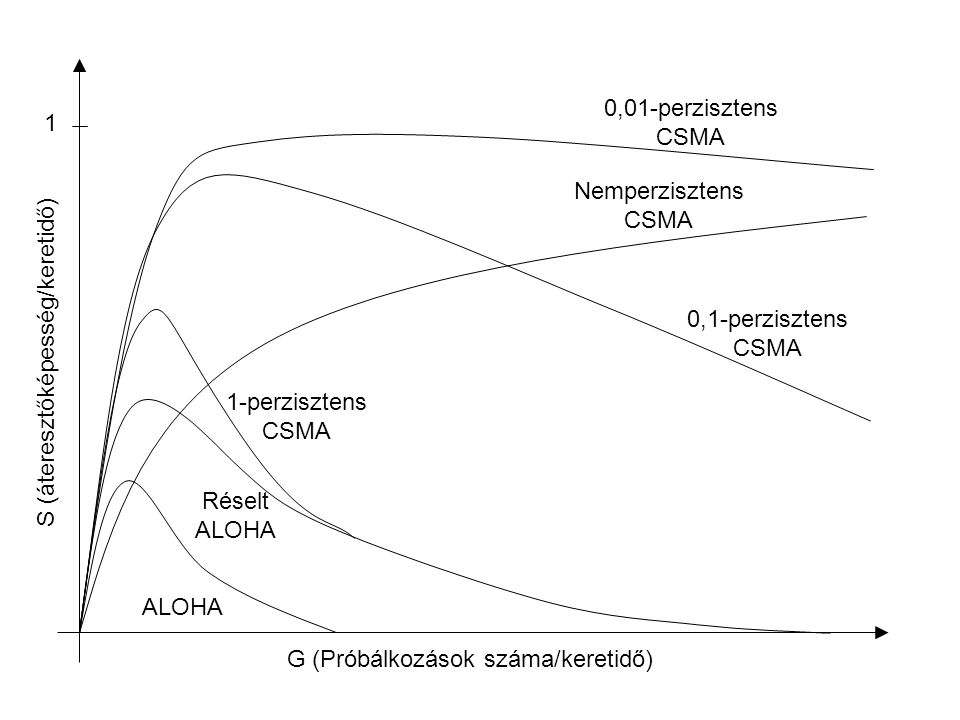
\includegraphics[width=0.55\textwidth]{img/aloha_csma.jpg}
%        	\caption{ALOHA és CSMA protokollok összehasonlítása}
        \end{figure}

    \subsubsection*{Verseny mentes protokollok}

    Motiváció: Az ütközések hátrányosan hatnak a rendszer teljesítményére, és a CSMA/CD nem mindenhol alkalmazható.\\

    \noindent N állomás van. Az állomások 0-ától N-ig egyértelműen sorszámozva vannak. Réselt időmodellt feltételezünk.
    \begin{itemize}[leftmargin=7.5mm]
        \renewcommand{\labelitemi}{$\vcenter{\hbox{\tiny$\bullet$}}$}
        \item \textbf{\small Egy helyfoglalásos protokoll} \\
        Ha az i-edik állomás küldeni szeretne, akkor az i-edik versengési időrésben egy 1-es bit elküldésével jelezheti. Így a versengési időszak végére minden állomás ismeri a küldőket. A küldés a sorszámok szerinti sorrendben történik meg.
        \item \textbf{\small Bináris visszaszámlálás protokoll} \\
        Minden állomás azonos hosszú bináris azonosítóval rendelkezik. A forgalmazni kívánó állomás elkezdi a bináris címét bitenként elküldeni a legnagyobb helyi értékű bittel kezdve. Az azonos pozíciójú bitek logikai VAGY kapcsolatba lépnek ütközés esetén. Ha az állomás nullát küld, de egyet hall vissza, akkor feladja a küldési szándékát, mert van nála nagyobb azonosítóval rendelkező küldő.
    \end{itemize}

    \paragraph*{Korlátozott verseny protokollok}

    Olyan protokoll, amely kis terhelés esetén versenyhelyzetes technikát használ a kis késleltetés érdekében, illetve nagy terhelés mellett ütközésmentes technikát alkalmaz a csatorna jó kihasználása érdekében.

    \paragraph*{\small Adaptív fabejárás}

    \begin{itemize}[leftmargin=7.5mm]
        \renewcommand{\labelitemi}{$\vcenter{\hbox{\tiny$\bullet$}}$}
        \item Minden állomást egy egyértelmű, bináris ID reprezentál.
        \item Az ID-k egy (bináris) fa leveleinek felelnek meg.
        \item Az időrések a fa egyes csomópontjaihoz vannak rendelve.
        \item Minden időrésben megvizsgáljuk az adott csomópont alatti részfát.
        \item A fa egy $u$ csomópontjánál 3 esetet különböztethetünk meg:
        \begin{itemize}[leftmargin=7.5mm]
            \renewcommand{\labelitemii}{$\vcenter{\hbox{\tiny$\circ$}}$}
            \item Egy állomás sem küld az $u$ részfában.
            \item Pontosan egy állomás küld az $u$ részfában.
            \item Több állomás küld az $u$ részfában. Ezt nevezzük kollíziónak.
        \end{itemize}
    \end{itemize}
    Kollízió esetén hajtsuk végre az ellenőrzést $u$ bal, és jobb oldali gyerekére egyaránt. Ezzel a módszerrel könnyen megállapítható, hogy melyik állomás küldhet az adott időszeletben.
        \begin{figure}[H]
            \centering
            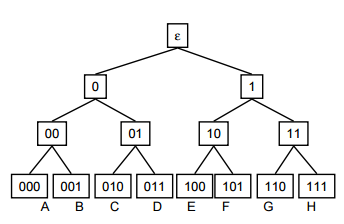
\includegraphics[width=0.5\textwidth]{img/adaptivfa.png}
            \caption{Adaptív fabejárás protokoll bináris fája}	
        \end{figure}

	\section*{3. Hálózati réteg}
		
    A hálózati réteg fő feladata a csomagok továbbítása a forrás és a cél között. Ez a legalacsonyabb olyan réteg, amely két végpont közötti átvitellel foglalkozik. Ismernie kell a kommunikációs alhálózat topológiáját. Ügyelni kell, hogy ne terheljen túl se bizonyos kommunikációs útvonalakat, se bizonyos routereket úgy, hogy mások tétlen maradnak.\\

    \noindent A szállítási réteg felé nyújtott szolgálatok:
    \begin{itemize}[leftmargin=7.5mm]
        \renewcommand{\labelitemi}{$\vcenter{\hbox{\tiny$\bullet$}}$}
        \item Függetlenek az alhálózatok kialakításától
        \item Eltakarják a jelen lévő alhálózatok számát, típusát és topológiáját
        \item A szállítási réteg számára rendelkezésre bocsájtott hálózati címek egységes számozási rendszert kell alkotnak
    \end{itemize}
	
    \subsection*{Forgalom irányítás típusai}

    \begin{itemize}[leftmargin=7.5mm]
        \renewcommand{\labelitemi}{$\vcenter{\hbox{\tiny$\bullet$}}$}
        \item \textbf{\small Hierarchikus forgalomirányítás}\\\\
        Routereket tartományokra osztjuk. A saját tartományát az összes router ismeri, de a többi belső szerkezetéről nincs tudomása. Nagy hálózatok esetén többszintű hierarchia lehet szükséges.
        \item \textbf{\small Adatszóró forgalomirányítás}\\\\
        Egy csomag mindenhová történő egyidejű küldése.
        \item \textbf{\small Többküldéses forgalomirányítás}\\\\
        Egy csomag meghatározott csoporthoz történő egyidejű küldése.
    \end{itemize}
\newpage
	\subsubsection*{Forgalom irányító algoritmusok}

     A hálózati réteg szoftverének azon része, amely azért a döntésért felelős, hogy a bejövő csomag melyik kimeneti vonalon kerüljön továbbításra. A folyamat két lépésre bontható:
     \begin{enumerate}
        \item Forgalomirányító táblázatok feltöltése és karbantartása.
        \item Továbbítás.
     \end{enumerate}

     A forgalomirányító algoritmusok osztályai:
     \begin{enumerate}
        \item Adaptív algoritmusok
        \begin{enumerate}
            \item távolság alapú
            \item kapcsolat alapú
        \end{enumerate}
        A topológia és rendszerint a forgalom is befolyásolhatja a döntést.
        \item Nem-adaptív algoritmusok \\
        Offline meghatározás, betöltés a routerekbe induláskor
     \end{enumerate}

    \paragraph*{Dijkstra algoritmus\\}

    A Dijkstra algoritmus egy statikus algoritmus, melynek célja két csomópont közötti legrövidebb út meghatározása.\\

    \noindent Minden csomópontot felcímkézünk a kezdőpontból az addig megtalált legrövidebb út távolságával. Kezdetben minden távolság végtelen, mivel nem ismerünk útvonalat.\\

    \noindent Az algoritmus működése során a címkék változhatnak az utak megtalálásával. Két fajta címkét különböztetünk meg: ideiglenes és állandó. Kezdetben minden címke ideiglenes. A legrövidebb út megtalálásakor a címke állandó címkévé válik, és továbbá nem változik.

    \paragraph*{Elárasztás algoritmus\\}

    Elárasztás algoritmusa egy statikus algoritmus.\\

    \noindent Minden bejövő csomagot minden kimenő vonalon továbbítunk kivéve azon, amin érkezett. Így azonban nagyon sok duplikátum keletkezne. Ezért
    \begin{itemize}[leftmargin=7.5mm]
        \renewcommand{\labelitemi}{$\vcenter{\hbox{\tiny$\bullet$}}$}
    	\item Ugrásszámlálót vezetünk be, melyet minden állomás eggyel csökkent. Ha 0-ra csökken, eldobják.
    	\item Az állomások nyilvántartják a már kiküldött csomagokat. Így egy csomagot nem küldenek ki többször.
    \end{itemize}

    \paragraph*{Elosztott Bellman-Ford algoritmus\\}

    \noindent Az Elosztott Bellman-Ford algoritmus adaptív, távolság alapú forgalomirányító algoritmus. Minden csomópont csak a közvetlen szomszédjaival kommunikálhat. Minden állomásnak van saját távolság vektora. Ezt periodikusan elküldi a direkt szomszédoknak. Minden router ismeri a közvetlen szomszédjaihoz a költséget. A kapott távolság vektorok alapján minden csomópont aktualizálja a saját vektorát.

    \paragraph{Kapcsolatállapot alapú forgalomirányítás\\}

    A kapcsolatállapot alapú forgalomirányító algoritmusnak a motivációja, hogy a távolság alapú algoritmusok lassan konvergáltak, illetve az eltérő sávszélek figyelembevétele. \\

    \noindent A kapcsolatállapot alapú forgalomirányító algoritmus lépései:
    \begin{enumerate}
    	\item Szomszédok felkutatása, és hálózati címeik meghatározása
    	\item Megmérni a késleltetést vagy költséget minden szomszédhoz
    	\item Egy csomag összeállítása a megismert információkból
    	\item Csomag elküldése az összes többi routernek
    	\item Kiszámítani a legrövidebb utat az összes többi routerhez.\\
    \end{enumerate}

	\paragraph*{Hálózati réteg az Interneten\\}

    A hálózati réteg szintjén az internet autonóm rendszerek összekapcsolt együttesének tekinthető. Nincs igazi szerkezete, de számos főbb gerinchálózata létezik.\\

    \noindent A gerinchálózatokhoz csatlakoznak a területi illetve regionális hálózatok. A regionális és területi hálózatokhoz csatlakoznak az egyetemeken, vállalatoknál és az internet szolgáltatóknál lévő LAN-ok. Az internet protokollja, az IP.\\

    \noindent Az Interneten a kommunikáció az alábbi módon működik:
        \begin{enumerate}
        	\item A szállítási réteg viszi az adatfolyamokat és datagramokra tördeli azokat.
        	\item Minden datagram átvitelre kerül az Interneten, esetleg menet közben kisebb egységekre darabolva.
        	\item A célgép hálózati rétege összeállítja az eredeti datagramot, majd átadja a szállítási rétegének.
        	\item A célgép szállítási rétege beilleszti a datagramot a vételi folyamat bemeneti adatfolyamába.
        \end{enumerate}

    \paragraph*{Internet Protokoll - IP\\}

    \begin{itemize}[leftmargin=7.5mm]
        \renewcommand{\labelitemi}{$\vcenter{\hbox{\tiny$\bullet$}}$}
        \item Az IP fejrésze:
    	\begin{itemize}
            \item verzió: IP melyik verzióját használja
            \item IHL: a fejléc hosszát határozza meg
            \item szolgálat típusa: szolgálati osztályt jelöl
            \item teljes hossz: fejléc és adatrész együttes hossza bájtokban
            \item azonosítás: egy datagram minden darabja ugyanazt az azonosításértéket hordozza.
            \item DF: "ne darabold" flag a routereknek
            \item MF: "több darab" flag minden darabban be kell legyen állítva, kivéve az utolsót.
            \item darabeltolás: a darab helyét mutatja a datagramon belül.
            \item élettartam: másodpercenként kellene csökkenteni a mező értékét, minden ugrásnál csökkentik eggyel az értékét
            \item protokoll: szállítási réteg protokolljának azonosítóját tartalmazza
            \item ellenőrző összeg: a routereken belüli rossz memóriaszavak által előállított hibák kezelésére használt ellenőrző összeg a fejrészre, amelyet minden ugrásnál újra kell számolni
            \item forrás cím és cél cím: IP cím
            \item opciók: következő verzió bővíthetősége miatt hagyták benne.
    	\end{itemize}
    	
    	\begin{figure}[H]
            \centering
            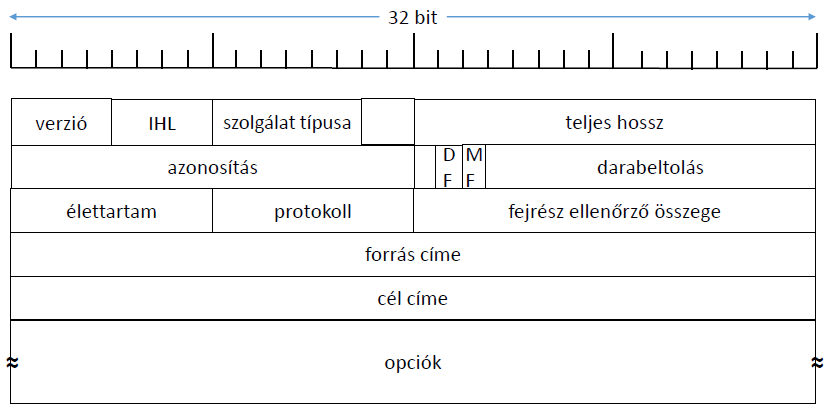
\includegraphics[width=0.75\textwidth]{img/ip_fejresz.png}
            \caption{IPv4 fejléce}
    	\end{figure}
    	
    	\item Az IP cím \\
        Minden hoszt és minden router az Interneten rendelkezik egy IP-címmel, amely a hálózat számát és a hoszt számát kódolja. 4 bájton ábrázolják az IP-címet. Az IP-t pontokkal elválasztott decimális rendszerben írják. (Például: 192.168.0.1)\\
        Van pár speciális cím (ábra \ref{fig:ip_spec_cimek}).

        \begin{figure}[H]
        	\centering
        	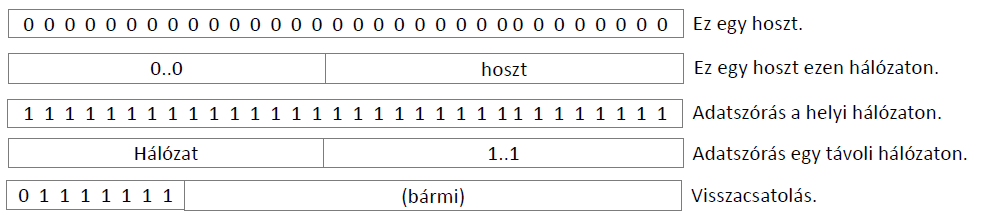
\includegraphics[width=0.8\textwidth]{img/ip_spec_cimek.png}
        	\caption{Speciális IP címek}
        	\label{fig:ip_spec_cimek}
        \end{figure}

        \paragraph*{Alhálózatok}

        Az azonos hálózatban lévő hosztok ugyanazzal a hálózatszámmal rendelkeznek. Egy hálózat belső felhasználás szempontjából több részre osztódhat, de a külvilág számára egyetlen hálózatként jelenik meg. Azonosításnál az alhálózati maszk ismerete kell a routernek. A forgalomirányító táblázatba a routereknél (hálózat,0) és (saját hálózat, hoszt) alakú bejegyzések. Ha nincs találat, akkor az alapértelmezett router felé továbbítják a csomagot.

        \paragraph*{IP címek fogyása}

        Az IP címek gyorsan fogytak. Megoldás: osztályok nélküli környezetek közötti forgalomirányítás (CIDR). A forgalomirányítás megbonyolódik: Minden bejegyzés egy 32-bites maszkkal egészül ki. Egy bejegyzés innentől egy hármassal jellemezhető: (ip-cím, alhálózati maszk, kimeneti vonal). Új csomag esetén a cél címből kimaszkolják az alhálózati címet, és találat esetén a leghosszabb illeszkedés felé továbbítják.

        Másik módszer a NAT, ami gyors javítás az IP címek elfogyásának problémájára. Az internet forgalomhoz minden cégnek egy vagy legalábbis kevés IP-címet adnak, míg vállalaton belül minden számítógéphez egyedi IP-címet használnak a belső forgalomirányításra: \\

        \begin{center}
            \renewcommand{\arraystretch}{2}
            $\begin{array}{r|r|r}
                10.0.0.0 & 10.255.255.255 & 16.777.216\ \text{egyedi cím} \\
                172.16.0.0 & 172.31.255.255 & 1.048.576\ \text{egyedi cím} \\
                192.168.0.0 & 192.168.255.255 & 65.536\ \text{egyedi cím} \\
            \end{array}$
            \renewcommand{\arraystretch}{1}
        \end{center}

        \paragraph*{IPv6:\\}

        Az IPv4-gyel szemben 16 bájt hosszú címeket használ; 8 darab, egyenként \\
        négy-négy hexadecimális számjegyből álló csoportként írjuk le. \\
        (Például: 8000:0000:0000:0000:0123:4567:89AB:CDEF) Az IP fejléc egyszerűsödött, amely lehetővé teszi a routereknek a gyorsabb feldolgozást. A biztonság irányába jelentős lépés történt.

        \begin{figure}[H]
        	\centering
        	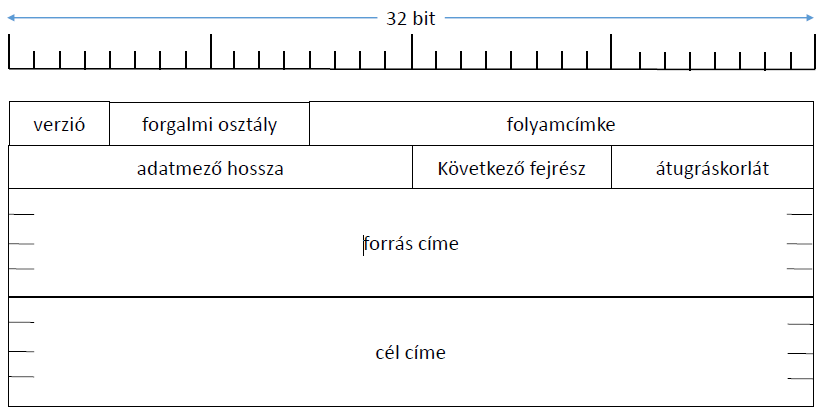
\includegraphics[width=0.65\textwidth]{img/ipv6.png}
        	\caption{IPv6 fejléce}
        \end{figure}

		\end{itemize}
\newpage
	\paragraph*{Protokollok\\}

	\begin{itemize}[leftmargin=7.5mm]
        \renewcommand{\labelitemi}{$\vcenter{\hbox{\tiny$\bullet$}}$}
        \item \textbf{\small Internet Control Message Protocol - ICMP} \\
        Feladata a váratlan események jelentése. Többféle ICMP-üzenetet definiáltak:
        \begin{itemize}[leftmargin=7.5mm]
            \renewcommand{\labelitemii}{$\vcenter{\hbox{\tiny$\circ$}}$}
            \item Elérhetetlen cél
            \item Időtúllépés
            \item Paraméterprobléma
            \item Forráslefojtás
            \item Visszhang kérés
            \item Visszhang válasz
            \item etc.
        \end{itemize}
        \item \textbf{\small Address Resolution Protocol - ARP} \\\\
        Feladata az IP cím megfeleltetése egy fizikai címnek. Egy "Kié a 192.60.34.12-es IP-cím?" csomagot küld ki az Ethernet-re adatszórással az alhálózaton. Minden egyes host ellenőrzi, hogy övé-e a kérdéses IP-cím. Ha egyezik az IP a hoszt saját IP-jével, akkor a saját Ethernet címével válaszol.
        \item \textbf{\small Reverse Address Resolution Protocol - RARP} \\\\
        Feladatat a fizikai cím megfeleltetése egy IP címnek. Az újonnan indított állomás adatszórással csomagot küld ki az Ethernetre: "A 48-bites Ethernet-címem 14.04.05.18.01.25. Tudja valaki az IP címemet?" Az RARP-szerver pedig válaszol a megfelelő IP címmel, mikor meglátja a kérést.
        \item \textbf{\small Open Shortest Path First - OSPF} \\\\
        Az OSPF az AS-eken (Autonomus System) belüli forgalomirányításért felel. A hálózat topológiáját térképezi fel, és érzékeli a változásokat. A topológiát egy súlyozott irányított gráffal reprezentálja, melyben legolcsóbb utakat keres.
        \item \textbf{\small Border Gateway Protocol - BGP} \\\\
        Feladata hogy a politikai szempontok szerepet játsszanak az AS-ek közötti forgalomirányítási döntésekben.\\\\
        {\small Például: Az IBM-nél kezdődő illetve végződő forgalom ne menjen át a Microsoft-on vagy Csak akkor haladjunk át Albánián, ha nincs más út a célhoz.}\\\\
        A BGP router szempontjából a világ AS-ekből és a közöttük átmenő vonalakból áll. (Két AS összekötött, ha van köztük a BGP-routereiket összekötő vonal.)\\
        Az átmenő forgalom szempontjából 3 féle hálózat van:
        \begin{itemize}
            \item Csonka hálózatok, amelyeknek csak egyetlen összeköttetésük van a BGP gráffal
            \item Többszörösen bekötött hálózatok, amelyeket használhatna az átmenő forgalom, de ezek ezt megtagadják
            \item Tranzit hálózatok, amelyek némi megkötéssel, illetve általában fizetség ellenében, készek kezelni harmadik fél csomagjait
        \end{itemize}
	\end{itemize}

	\section*{4. Szállítói réteg}

    \begin{itemize}
        \item A szállítási réteg biztosítja, hogy a felhasználók közötti adatátvitel transzparens (átlátszó) legyen.
        \item A réteg biztosítja, és ellenőrzi egy adott kapcsolat megbízhatóságát.
        \item Az alkalmazási rétegtől kapott adat elejére egy úgynevezett fejlécet csatol, mely jelzi, hogy melyik szállítási rétegbeli protokollal küldik az adatot.
        \item Néhány protokoll kapcsolat orientált. Ez azt jelenti, hogy a réteg nyomon követi az adatcsomagokat, és hiba esetén gondoskodik a csomag vagy csomagok újraküldéséről.
    \end{itemize}
			
	\subsubsection*{Kapcsolat nélküli és kapcsolatorientált}

    \noindent A kapcsolatorientált protokoll elfedi az alkalmazások előtt az átvitel esetleges hibáit, nem kell törődnünk az elveszett, vagy duplán megérkezett, illetve sérült csomagokkal, és azzal sem, hogy milyen sorrendben érkeztek meg. Viszont ez rontja a teljesítményét.

	\noindent Kapcsolat nélküli esetben nincs szükség az adat keretekre bontására, és nincs  csomagújraküldés.

	\paragraph*{Megbízhatóság}

	A megbízhatóság ismérvei:
	\begin{itemize}
        	\item Minden csomag megérkezése nyugtázásra kerül.
        	\item A nem nyugtázott adatcsomagokat újraküldik.
        	\item A fejléchez és a csomaghoz ellenőrzőösszeg van rendelve.
        	\item A csomagokat számozza, és a fogadónál sorba rendezésre kerülnek a csomagok a sorszámaik alapján.
        	\item Duplikátumokat törli.
	\end{itemize}

	\subsubsection*{Torlódásfelügyelet}

	Minden hálózaton  korlátos az átviteli sávszélessége. Ha több adatot vezetünk a hálózatba, akkor az torlódáshoz (congestion) vezet, vagy akár a hálózat összeomlásához (congestive collapse). Következmény: Az adatcsomagok nem érkeznek meg.\\

	\noindent \textbf{Lavina jelenség:} A hálózat túlterhelése csomagok elvesztését okozza, ami csomag újraküldését eredményezi. Az újraküldés tovább növeli a hálózat terhelését így még nagyobb lesz csomagvesztés. Ez még több újraküldött csomagot eredményez. ... \\
	A torlódás felügyelet feladata a lavina jelenség elkerülése.

	\paragraph*{Követelmények a torlódásfelügyelettel szemben}

	\begin{itemize}
		\item Hatékonyság: Az átvitel nagy, míg a késés kicsi.
		\item Fairness: Minden folyamat megközelítőleg azonos részt kap a sávszélességből. (Priorizálás lehetősége fennáll)
	\end{itemize}

	\paragraph*{A torlódásfelügyelet eszközei}
	\begin{itemize}
		\item Kapacitásnövelés
		\item Erőforrás foglalás és hozzáférés szabályzás
		\item Terhelés csökkentése és szabályzása
	\end{itemize}

	\paragraph*{Stratégiák}
	\begin{itemize}
		\item \textbf{Csúszóablak} \\
            Adatráta szabályozása ablak segítségével. A fogadó határozza meg az ablak (wnd) méretét. Ha a fogadási puffere tele van, lecsökkenti 0-ra, egyébként \textgreater0-t küld. A küldő nem küld több csomagot, ha az elküldött még nem nyugtázott csomagok száma elérte az ablak méretét. 	
			\begin{figure}[H]
        \centering
        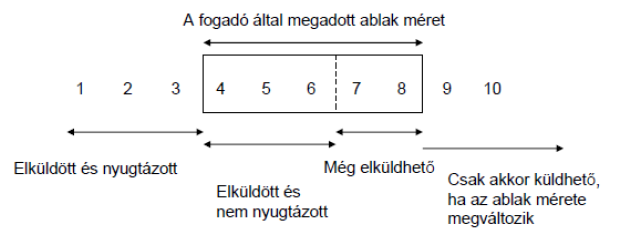
\includegraphics[width=0.6\textwidth]{img/csuszoablak.png}
        \caption{Csúszóablak}
			\end{figure}
		\item \textbf{Slow-start} \\
        A küldőnek nem szabad a fogadó által küldött ablakméretet azonnal kihasználni. Meghatároz egy másik ablakot (cwnd - Congestion Window), melyet ő választ. Ezután végül amiben küld: min\{wnd, cwnd\}. Kezdetben cwnd = MSS (Maximum Segment Size). Minden csomagnál a megkapott nyugta után növeli: cwnd = cwnd + MSS (azaz minden RTT után duplázódik). Ez addig megy, míg a nyugta egyszer kimarad.
		\item \textbf{TCP-Nagle} \\
		Biztosítani kell, hogy a kis csomagok időben egymáshoz közel kerüljenek kiszállításkor, illetve hogy sok adat esetén a nagy csomagok részesüljenek előnyben.
        \begin{itemize}
            \item A kis csomagok nem kerülnek kiküldésre, míg nyugták hiányoznak (egy csomag kicsi, ha az adathossz \textless MSS).
            \item Ha a korábban küldött csomag nyugtája megérkezik, küldi a következőt.
        \end{itemize}
		\item \textbf{TCP Tahoe és Reno} \\
        A TCP csúszóablakot és a Slow-start mechanizmusát is használja. Habár a kezdő ráta kicsi, az ablak mérete rohamosan nő. Amikor a cwnd eléri az ssthresh (slow start threshold) értéket átvált torlódás elkerülési állapotba. A TCP Tahoe és Reno torlódás elkerülési algoritmusok. A két algoritmus abban különbözik, hogy hogyan detektálják és kezelik a csomag vesztést. \\

		\noindent \emph{TCP Tahoe}: A torlódás detektálására egy időzítőt állít a várt nyugta megérkezésére.
		\begin{itemize}
			\item Kapcsolatfelvételkor:
            \begin{itemize}
                \item cwnd = MSS,
                \item ssthresh = $2^{16}$
            \end{itemize}
			\item Csomagvesztésnél : Multiplicative decrease
            \begin{itemize}
                \item cwns = MSS,
                \item ssthresh = max $\left\{2MSS, \frac{min\{cwnd, wnd\}}{2}\right\}$
            \end{itemize}
			\item cwnd $\leq$\ ssthresh : Slow-start \\
            cwnd = cwnd + MSS
			\item cwnd $>$ ssthresh : Additive Increase \\
            cwnd = cwnd + MSS$\frac{MSS}{cwnd}$
		\end{itemize}
		\noindent \emph{TCP Reno}: A torlódás detektálásához időzítőt és gyors újraadást is használ. [Gyors újraadás: ugyanazon csomaghoz 3 nyugta duplikátum érkezik (4 azonos nyugta), akkor újraküldi a csomagot és Slow-start fázisba lép.] \\\\
		Gyors újraadás után:
        \begin{itemize}
            \item ssthresh = max\{$\frac{min\{wnd,cwnd\}}{2}$, 2MSS\},
            \item cwnd = sstresh + 3MSS.
        \end{itemize}
		Gyors visszaállítás a gyors újraadás után minden további nyugta után növeli a rátát:
        \begin{itemize}
            \item cwnd = cwnd + MSS.
        \end{itemize}
	\end{itemize}

	\noindent Hatékonyság és Fairness: \\
    Az átvitel maximális, ha a terhelés a hálózat kapacitását majdnem eléri. Ha a terhelés tovább nő, túlcsordulnak a pufferek, csomagok vesznek el, újra kell küldeni, drasztikusan nő a válaszidő. Ezt a torlódásnak nevezzük. Ezért a maximális terhelés helyett, ajánlatos a hálózat terhelését a könyök közelében beállítani. Itt a válaszidő csak lassan emelkedik, míg az adatátvitel már a maximum közelében van.\\

	\noindent Egy jó torlódáselkerülési (angolul congestion avoidance) stratégia a hálózat terhelését a könyök közelében tartja: \textit{hatékonyság}. Emellett fontos, hogy minden résztvevőt egyforma rátával szolgáljunk ki: \textit{fairness}\\

	\noindent Jelölje az $i$-edik résztvevő adatrátáját a $t$ időpontban $x_i(t)$.
	Minden résztvevő aktualizálja az adatrátáját a $t+1$-ik fordulóban:
	\begin{align*}
		x_i(t+1) = f_0(t) \quad  ha \ \sum_{i=1}^{n}x_i(t) \leq K \\
		x_i(t+1) = f_1(t) \quad  ha \ \sum_{i=1}^{n}x_i(t) > K
	\end{align*}
	ahol $f_0(x) = a_I + b_Ix$ a növelési, $f_1(x) = a_D + b_Dx$ a csökkentési stratégia.

	\paragraph*{Speciális esetek}

	\begin{itemize}
		\item \textbf{M}ultiplcative \textbf{I}ncrease \textbf{M}ultiplcative \textbf{D}ecrease - MIMD:
		\begin{align*}
			f_0(x) = b_Ix \quad (b_I > 1) \qquad
            f_1(x) = b_Dx \quad (b_D < 1)
		\end{align*}
	   \item \textbf{A}dditive \textbf{I}ncrease \textbf{A}dditive \textbf{D}ecrease - AIAD:
	   \begin{align*}
		  f_0(x) = a_I+x \quad (a_I > 0) \qquad
		  f_1(x) = a_D+x \quad (a_D < 0)        	
	   \end{align*}
	   \item \textbf{A}dditive \textbf{I}ncrease \textbf{M}ultiplcative \textbf{D}ecrease - AIMD:
	   \begin{align*}
    		f_0(x) = a_I+x \quad (a_I > 0) \qquad
            f_1(x) = b_Dx \quad (b_D < 1)
	   \end{align*}
    \end{itemize}

    \paragraph{Multiplexálás, demultiplexálás}

    Multiplexelés alatt a telekommunikációban azt az eljárást értik, amikor két vagy több csatornát összefognak egy csatornába úgy, hogy az inverz multiplexelés művelettel, vagy demultiplexeléssel, vagy demuxálással elő tudják állítani az eredeti csatornákat. Az eredeti csatornák egy úgynevezett kódolási sémával azonosíthatóak.

    \paragraph{Interakciós modellek}

    \begin{itemize}
        \item \textbf{\small Kétirányú bájtfolyam} \\
        {\small Az adatok két egymással ellentétes irányú bájt-sorozatként kerülnek átvitelre. A tartalom nem interpretálódik Az adatcsomagok időbeli viselkedése megváltozhat: átvitel sebessége növekedhet, csökkenhet, más késés, más sorrendben is megérkezhetnek. Megpróbálja az adatcsomagokat időben egymáshoz közel kiszállítani. Megpróbálja az átviteli közeget hatékonyan használni.}
        	
        \item \textbf{\small RPC} \\
        {\small A távoli gépen futtatandó eljárás eléréséhez hálózati kommunikációra van szükség, ezt az eljáráshívási mechanizmust az RPC (Remote Procedure Call) fedi el.}

        A hívás lépései:
        \begin{enumerate}
            \small
            \item A kliensfolyamat lokálisan meghívja a	klienscsonkot.
            \item Az becsomagolja az eljárás azonosítóját és paramétereit, meghívja az OS-t.
            \item Az átküldi az üzenetet a távoli OS-nek.
            \item Az átadja az üzenetet a szervercsonknak.
            \item Az kicsomagolja a paramétereket, átadja a szervernek.
            \item A szerver lokálisan meghívja az eljárást, megkapja a visszatérési értéket.
            \item Ennek visszaküldése a klienshez hasonlóan zajlik, fordított irányban.
        \end{enumerate}
        \begin{figure}[H]
        	\centering
        	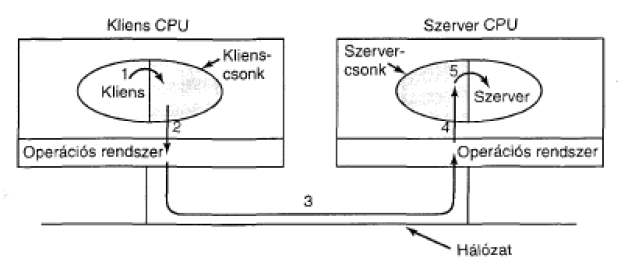
\includegraphics[width=0.6\textwidth]{img/rpc.png}
        	\caption{RPC}
        \end{figure}
    \end{itemize}

	\subsection*{Protokollok\\}

	\subsubsection*{TCP}

    \begin{itemize}
        \item Megbízható adatfolyam létrehozása két végpont között
        \item Az alkalmazási réteg adatáramát osztja csomagokra
        \item A másik végpont a csomagok fogadásról nyugtát küld
    \end{itemize}

    \noindent A TCP fejléc tartalma:\\

    \renewcommand{\arraystretch}{2}
    {\footnotesize
      $\begin{array}{l|c|l}
        \text{Küldő port} & \text{16 bit} & \text{A küldő folyamatot azonosítja} \\ \hline
        \text{Cél port} & \text{16 bit} & \text{A címzett folyamat azonosítója} \\ \hline
        \text{Sorszám} & \text{32 bit} & \makecell[l]{\text{Az első adatbájt sorszáma az aktuális szegmensen belül}.\\\text{Ha a SYN jelzőbit értéke 1, akkor ez a sorszám a kezdeti sorszám, azaz}\\\text{az első adatbájt sorszáma a kezdeti sorszám + 1 lesz.}} \\ \hline
        \text{Nyugtaszám} & \text{32 bit} & \makecell[l]{\text{Ha az ACK jelzőbit értéke 1, akkor}\\\text{a fogadó által következőnek fogadni kívánt sorszámot tartalmazza.}\\\text{Minden kapcsolat felépítés esetén elküldésre kerül.}} \\ \hline
        \text{Fejléc hossza} & \text{4 bit} & \text{A TCP fejléc hossza 32-bites egységekben.} \\ \hline
        \text{Ablak} & \text{16 bit} & \makecell[l]{\text{A nyugtázott bájttal kezdődően hány bájtot lehet elküldeni.}\\\text{(A 0 érték is érvényes.)}} \\ \hline
        \text{Ellenőrzőösszeg} & \text{16 bit} & \text{Az adat-, fej-, és pszeudofejrész ellenőrzésére.} \\ \hline
        \text{Opciók} & \text{0-40 bájt} & \makecell[l]{\text{A szabványos fejlécen kívüli lehetőségekre tervezték.}\\\text{Legfontosabb ilyen lehetőség az MSS, azaz}\\\text{a legnagyobb szegmens méret megadása.}\\\text{További opciók: MD5-aláírás, TCP-AO, "usertimeout", stb.}} \\ \hline
        \text{Sürgősségi mutató} & \text{16 bit} & \makecell[l]{\text{A sürgős adat bájtban mért helyét jelzi a}\\\text{jelenlegi bájtsorszámhoz viszonyítva.}} \\ \hline
        \text{Jelző bitek} & &
            \renewcommand{\arraystretch}{1}
              \begin{array}{l}
                \text{URG – Sürgős jelzőbit.} \\
                \text{ACK – nyugta jelzés.} \\
                \text{PSH – Az jelzi, hogy gyors adattovábbítás kell a felhasználói rétegnek.} \\
                \text{RST – Kapcsolat egyoldalú bontását jelzi.} \\
                \text{SYN – Sorszám szinkronizációtjelez.} \\
                \text{FIN – Adatfolyam végét jelzi.} \\
              \end{array}
        \renewcommand{\arraystretch}{2}
      \end{array}$
      }
    \renewcommand{\arraystretch}{1}

    \begin{figure}[H]
        \centering
        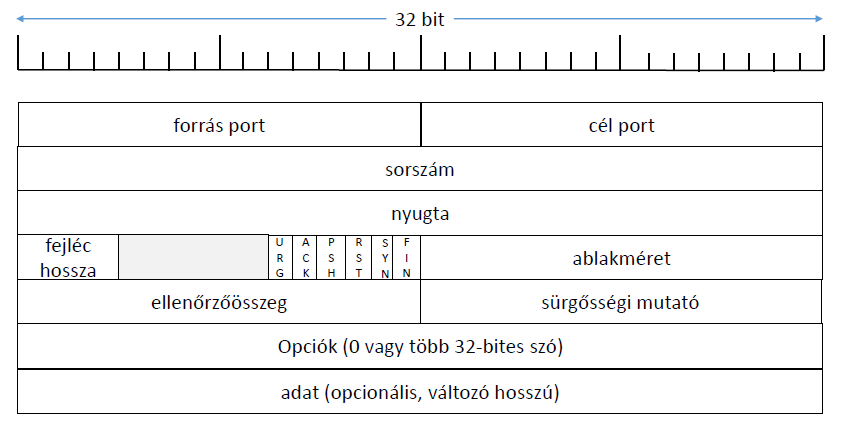
\includegraphics[width=0.6\textwidth]{img/tcp_fejlec.png}
        \caption{TCP Fejléc}
    \end{figure}
    \noindent TCP jellemzői:
    \begin{itemize}
        \item Kapcsolatorientált
        \item Megbízható
        \item Kétirányú bájtfolyam
    \end{itemize}

	\subsubsection*{UDP}

    Az UDP egy kapcsolat nélküli protokoll. A kommunikáció UDP csomagokkal (packet) történik, és a csomagok megérkezése nem garantált (elveszhetnek útközben). Továbbá, mivel az egyes csomagok akár más-más útvonalon is eljuthatnak a célhoz, a csomagok megérkezésének sorrendje is eltérhet a küldési sorrendtől.

    \begin{itemize}
        \item Egyszerű, nem megbízható szolgáltatás csomagok küldésére
        \item Az alkalmazási réteg határozza meg a csomag méretét
        \item Az inputot egy datagrammá alakítja	
    \end{itemize}
    Összeköttetés nélküli protokoll. Olyan szegmenseket használ az átvitelhez, amelyek egy 8 bájtos fejrészből, valamint a felhasználói adatokból állnak.\\

    \noindent A fejrész tartalmaz:
    \begin{itemize}
        \item egy forrásportot(2 bájt)
        \item egy célportot(2 bájt)
        \item egy UDP szegmens hossz értéket (2 bájt)
        \item egy UDP ellenőrzőösszeget (2 bájt)		
    \end{itemize}
    Az UDP nem végez forgalomszabályozást, hibakezelést vagy újraküldést egy rossz szegmens fogadása után. \\

    \noindent Kliens-szerver alkalmazások esetén kifejezetten hasznos lehet az UDP a rövid üzenetek miatt. \\

    \noindent UDP-t alkalmaznak például olyan esetekben, ahol egy csomagot érdemes inkább eldobni, mint várni annak újraküldésére. \\

    \noindent Ilyen lehet például: video-streaming, voice-over-IP alkalmazások (pl. internetes telefon), illetve bizonyos online játékok.
		
\end{document} 